% =====================================================================
% TECHNICAL REPORT - Todorut Aurel-Dan, group 30434
% Compile:  pdflatex technical_report.tex   (run it twice, for the contents)
% Figures are expected in ./figures/
% =====================================================================
\documentclass[11pt,a4paper]{article}
\usepackage[utf8]{inputenc}
\usepackage[T1]{fontenc}
\usepackage[english]{babel}
\usepackage[margin=2.5cm]{geometry}
\usepackage{graphicx}
\usepackage{booktabs}
\usepackage{amsmath}
\usepackage{amssymb}
\usepackage{xcolor}
\usepackage{fancyhdr}
\usepackage{enumitem}
\usepackage[hidelinks]{hyperref}
\usepackage{caption}
\usepackage{float}
\usepackage[section]{placeins}
\usepackage{array}
\graphicspath{{figures/}}
\captionsetup{font=small}
\setlist{itemsep=2pt, topsep=3pt}
\setlength{\parskip}{4pt}
\pagestyle{fancy}
\fancyhf{}
\fancyhead[L]{\small Technical report}
\fancyhead[R]{\small Todoruț Aurel-Dan, group 30434}
\fancyfoot[C]{\small \thepage}
\newcommand{\code}[1]{\texttt{#1}}

\title{\vspace{-1.5cm}\textbf{Technical Report}\\[0.3cm]
\large Deep Learning for Image Classification and\\Liver and Tumour Segmentation in CT}
\author{Todoruț Aurel-Dan\\[2pt]
\small Faculty of Automation and Computer Science, Technical University of Cluj-Napoca\\
\small Group 30434 \quad--\quad Tutor: Conf.dr.ing. Tiberiu Marita}
\date{Internship period: 13.07.2026 -- 21.08.2026}

\begin{document}
\maketitle
\thispagestyle{fancy}

\begin{abstract}
\noindent This report documents the technical work done during my internship. It
covers two projects, both written from scratch in PyTorch. The first is image
classification on CIFAR-10: a configurable convolutional network run on three
tasks (2, 6 and 10 classes), reaching 88.25\% and 88.85\% test accuracy on the
binary and ten-class tasks, followed by ten single-change experiments, an
overfitting experiment and Grad-CAM explanations. The second is semantic
segmentation of the liver and liver tumours in abdominal CT slices from the LiTS
dataset, where I implemented a U-Net and an Attention U-Net and compared them
under identical conditions. The two reach a foreground Dice of 0.8222 and 0.8247,
a difference too small to be meaningful. The report also describes the data
problems found along the way, the evaluation choices, an analysis of what the
attention gates learned, and the tools built to view a whole patient in 3D and
export it to 3D Slicer.
\end{abstract}

\tableofcontents
\newpage

% =====================================================================
\section{Introduction}
% =====================================================================

The internship had two parts. In the first one I built an image classifier to
learn the full deep learning workflow on a small and well known problem. In the
second one I used what I learned on a harder, real problem: finding the liver
and liver tumours in CT scans, pixel by pixel.

For both projects I wrote everything myself: configuration, data loading,
models, loss, training loop, evaluation, figures and checking tools. No
high-level training framework or segmentation library was used. The goal was not
only to get good numbers, but to be able to explain where each number comes from
and whether it can be trusted.

The report is organised by topic rather than by week. Section~\ref{sec:env}
describes the environment, Section~\ref{sec:cls} the classification project,
Section~\ref{sec:seg} the segmentation project, Section~\ref{sec:eng} the
engineering problems and how they were found, and Section~\ref{sec:lim} the
limitations. The weekly diary is in the separate internship notebook.

% =====================================================================
\section{Development environment}\label{sec:env}
% =====================================================================

\subsection{Software}

Each project has its own Miniconda environment (\code{cls} and \code{seg}) with
Python 3.12 and PyTorch built for CUDA 12.6. The main libraries are
\code{numpy}, \code{pillow}, \code{matplotlib}, \code{scikit-learn}
(classification metrics), \code{scikit-image} (3D surfaces) and \code{nibabel}
(medical image export). PyCharm was the editor and both projects are kept in git.
Model weights are not committed, but every run folder keeps its exact
configuration, training history and test metrics as JSON, so every number in this
report can be traced back to a file.

All code is run from the project root as a module (\code{python -m src.train}).
This avoids a problem I hit early: marking \code{src/} as a source root in the IDE
put \code{src} on the Python path, which made \code{src/utils} visible as a
top-level package called \code{utils} and caused import confusion with
\code{torch.utils}.

\subsection{Hardware}

\begin{table}[H]
\centering\small
\begin{tabular}{lll}
\toprule
\textbf{Machine} & \textbf{GPU} & \textbf{Used for} \\
\midrule
Laptop, Windows 11 & NVIDIA RTX 3050 Laptop & classification, first segmentation runs \\
Workstation, Linux (remote) & NVIDIA RTX 2070 & final segmentation runs \\
\bottomrule
\end{tabular}
\caption{Machines used.}
\end{table}

On the laptop one segmentation epoch took about 6 minutes, with GPU utilisation
around 68\% and temperature at 84--86\,\textdegree C. The GPU was waiting for data
and was also thermally limited. On Windows the data loader could not use worker
processes (see Section~\ref{sec:eng}), so loading happened in the main process.
On the Linux workstation, with several workers, utilisation reached 98\% at
66\,\textdegree C. Training ran inside \code{tmux} so that it survived the remote
connection dropping.

% =====================================================================
\section{Project 1: image classification on CIFAR-10}\label{sec:cls}
% =====================================================================

\subsection{Data}

CIFAR-10 has 60{,}000 colour images of $32\times32$ pixels in 10 classes: 50{,}000
for training and 10{,}000 for testing. It has no validation set, so 10\% of the
training images are held out for validation. The test set is used only once, at
the end, never to choose settings.

The set of classes is a configuration option, so the same code runs three tasks:

\begin{table}[H]
\centering\small
\begin{tabular}{llrr}
\toprule
\textbf{Task} & \textbf{Classes} & \textbf{Train + val} & \textbf{Test} \\
\midrule
binary & cat, dog & 10{,}000 & 2{,}000 \\
animals & bird, cat, deer, dog, frog, horse & 30{,}000 & 6{,}000 \\
multiclass & all 10 & 50{,}000 & 10{,}000 \\
\bottomrule
\end{tabular}
\caption{The three classification tasks. For the subsets, the original labels are
remapped to $0 \dots K-1$.}
\end{table}

Images are normalised per channel with the CIFAR-10 mean
$(0.4914, 0.4822, 0.4465)$ and standard deviation $(0.2470, 0.2435, 0.2616)$.
Augmentation, applied to the training set only, is a random $32\times32$ crop
from the image padded by 4 pixels, plus a random horizontal flip.

\subsection{Model}

The network is built from repeated convolution blocks. Each block has two
$3\times3$ convolutions, each followed by batch normalisation and ReLU, and ends
with $2\times2$ max pooling, which halves the resolution. The number of filters
doubles every block. After the last block, global average pooling reduces each
feature map to one number, then a fully connected layer of 256 units with ReLU
and dropout, and a final linear layer with one output per class. Convolutions use
Kaiming initialisation; because batch normalisation follows each convolution,
the convolutions have no bias.

\begin{table}[H]
\centering\small
\begin{tabular}{lllr}
\toprule
\textbf{Stage} & \textbf{Operation} & \textbf{Output} & \textbf{Parameters} \\
\midrule
input & & $3\times32\times32$ & \\
block 1 & 2$\times$(conv $3\times3$, BN, ReLU), max pool & $32\times16\times16$ & 10{,}208 \\
block 2 & 2$\times$(conv $3\times3$, BN, ReLU), max pool & $64\times8\times8$ & 55{,}552 \\
block 3 & 2$\times$(conv $3\times3$, BN, ReLU), max pool & $128\times4\times4$ & 221{,}696 \\
pooling & global average pool & 128 & 0 \\
hidden & linear, ReLU, dropout 0.3 & 256 & 33{,}024 \\
output & linear & $K$ & $257K$ \\
\midrule
\multicolumn{3}{l}{total, $K=2$ / 6 / 10} & 320{,}994 / 322{,}022 / 323{,}050 \\
\bottomrule
\end{tabular}
\caption{The default classification network. Depth, width, dropout and batch
normalisation are all configuration options, which is what makes the experiments
in Section~\ref{sec:cls_exp} possible.}
\label{tab:cls_arch}
\end{table}

Global average pooling instead of flattening keeps the fully connected part
small: flattening $128\times4\times4$ into a 256-unit layer would need 524{,}544
weights on its own, more than the whole network has now.

\subsection{Training}

\begin{table}[H]
\centering\small
\begin{tabular}{ll}
\toprule
\textbf{Setting} & \textbf{Value} \\
\midrule
loss & cross-entropy \\
optimiser & Adam, learning rate $10^{-3}$, weight decay $5\times10^{-4}$ \\
learning rate schedule & cosine annealing to zero over the run \\
batch size & 128 \\
epochs & 40 (binary), 50 (animals, multiclass) \\
early stopping & patience 8 epochs on validation accuracy \\
model selection & checkpoint with the best validation accuracy \\
seed & 42 \\
\bottomrule
\end{tabular}
\caption{Classification training setup.}
\end{table}

\subsection{Metrics}

On the test set I compute accuracy, balanced accuracy (the mean of the per-class
recalls), macro F1, the confusion matrix and, for the binary task, ROC-AUC. The
test sets are balanced, so accuracy and balanced accuracy agree here; they would
not on unbalanced data, which is exactly the situation in the segmentation
project.

\subsection{Baseline results}

\begin{table}[H]
\centering\small
\begin{tabular}{lrrrrrr}
\toprule
\textbf{Task} & \textbf{Epochs} & \textbf{Best epoch} & \textbf{Val acc}
& \textbf{Test acc} & \textbf{Macro F1} & \textbf{Minutes} \\
\midrule
binary     & 40 & 34 & 0.8850 & 0.8825 & 0.8825 & 2.9 \\
animals    & 50 & 48 & 0.8713 & 0.8680 & 0.8680 & 12.4 \\
multiclass & 50 & 43 & 0.8924 & 0.8885 & 0.8881 & 19.1 \\
\bottomrule
\end{tabular}
\caption{Baseline results on the test sets. Binary ROC-AUC is 0.9475.}
\label{tab:cls_base}
\end{table}

The ten-class task scores \emph{higher} than the six-class task. The four extra
classes are vehicles (airplane, automobile, ship, truck), which are easy to tell
apart from animals and from each other: automobile recall is 0.952 and ship 0.943.
The six-class task keeps only the animals, which look much more alike. More
classes does not automatically mean a harder problem; it depends on which
classes.

The per-class recalls show the same thing from another side. In both the animal
and the ten-class task, \textbf{cat} is the weakest class (0.778 and 0.750), and
the most frequent single mistake is a cat predicted as a dog (108 and 102 test
images). In the binary task the matrix is $[[896, 104], [131, 869]]$, so cat
recall is 0.896 and dog recall 0.869: errors in both directions, roughly
balanced.

\begin{figure}[H]
\centering
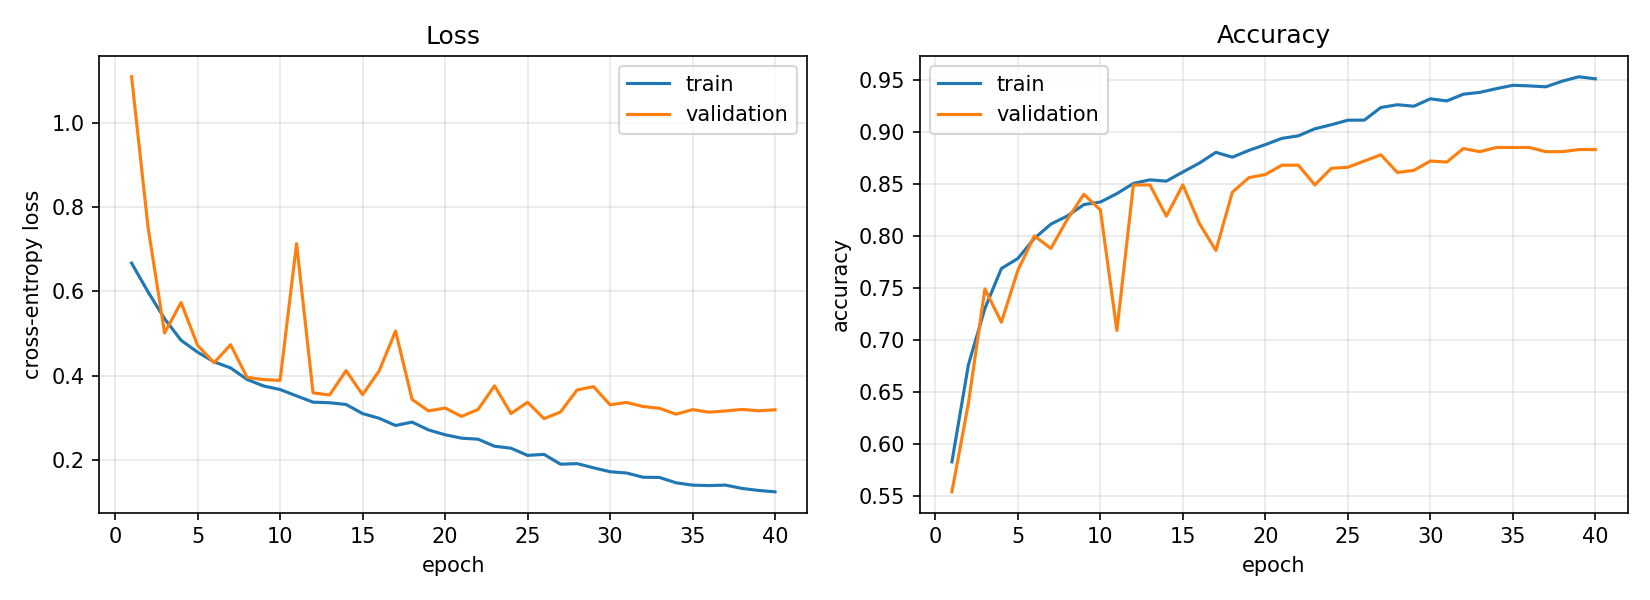
\includegraphics[width=0.56\textwidth]{cls_curves_binary.png}\hfill
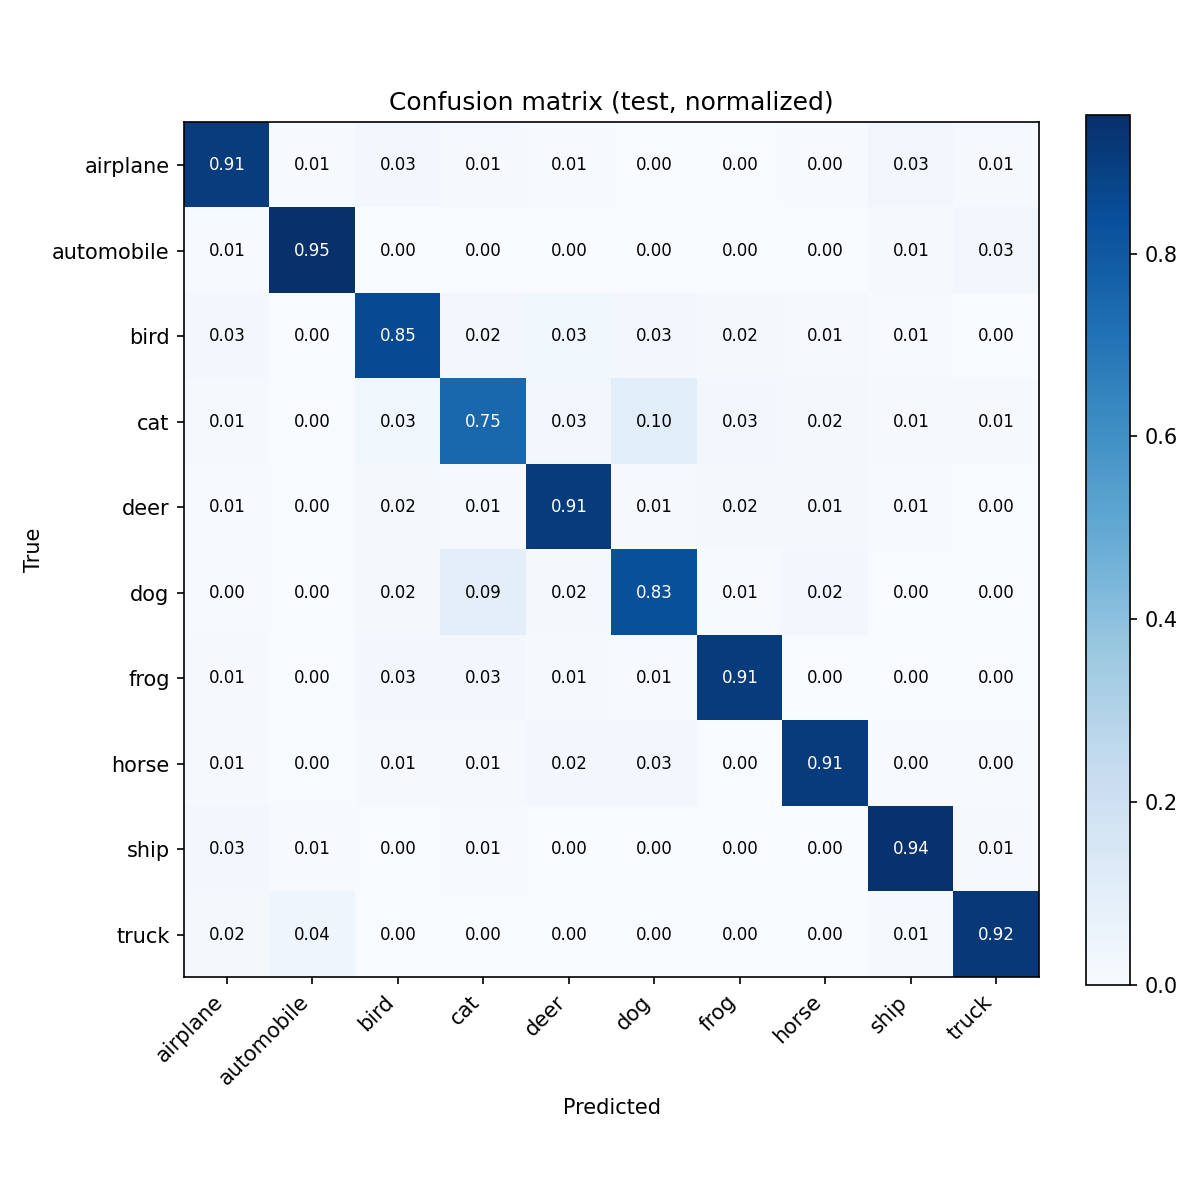
\includegraphics[width=0.40\textwidth]{cls_confusion_multi.png}
\caption{Left: training curves for the binary task. Right: normalised confusion
matrix for the ten-class task. The darkest off-diagonal cells are among the
animal classes, especially cat and dog.}
\end{figure}

\subsection{Experiments: which parts of the network matter}\label{sec:cls_exp}

To see what each design choice contributes, I trained ten variants of the binary
model, each changing exactly one thing. All were trained for 20 epochs so they
are comparable with each other. Because of the shorter budget the baseline here
scores 0.8575 instead of 0.8825; what matters is the difference between rows.

\begin{table}[H]
\centering\small
\begin{tabular}{llrrr}
\toprule
\textbf{Variant} & \textbf{What changed} & \textbf{Params}
& \textbf{Test acc} & \textbf{vs baseline} \\
\midrule
baseline         & 3 blocks, 32 filters, dropout 0.3, aug. & 320{,}994 & 0.8575 & -- \\
no\_dropout      & dropout 0 instead of 0.3        & 320{,}994   & \textbf{0.8720} & $+0.0145$ \\
wide\_64         & 64 base filters                 & 1{,}212{,}610 & 0.8695 & $+0.0120$ \\
deep\_4blocks    & 4 blocks instead of 3           & 1{,}239{,}522 & 0.8630 & $+0.0055$ \\
label\_smooth    & label smoothing 0.1             & 320{,}994   & 0.8580 & $+0.0005$ \\
convdrop         & spatial dropout 0.1 per block   & 320{,}994   & 0.8550 & $-0.0025$ \\
sgd              & SGD with momentum instead of Adam & 320{,}994 & 0.8440 & $-0.0135$ \\
no\_augment      & no random crop or flip          & 320{,}994   & 0.8410 & $-0.0165$ \\
shallow\_2blocks & 2 blocks instead of 3           & 82{,}914    & 0.8130 & $-0.0445$ \\
no\_batchnorm    & batch normalisation removed     & 320{,}546   & \textbf{0.7735} & $\mathbf{-0.0840}$ \\
\bottomrule
\end{tabular}
\caption{Single-change experiments on the binary task, 20 epochs each.}
\label{tab:cls_exp}
\end{table}

\begin{itemize}
  \item \textbf{Batch normalisation matters most.} Removing it costs 8.4 points,
        more than all the other changes combined. It removes only 448
        parameters, so this is not about capacity: it is about how easy the
        network is to optimise.
  \item \textbf{Dropout was hurting.} With augmentation already on and a network
        this small, dropout 0.3 was too much regularisation. Turning it off
        gained 1.5 points.
  \item \textbf{Depth matters more than width.} Going from 3 to 2 blocks costs
        4.5 points and removes 74\% of the parameters. Doubling the filters
        gains only 1.2 points for almost four times the parameters.
  \item \textbf{Augmentation is worth 1.7 points}, and Adam beat SGD with momentum
        at the same learning rate schedule within 20 epochs.
\end{itemize}

One limitation: each variant was trained once. Differences below about one
point (label smoothing, spatial dropout) are within what a different random seed
could change.

\subsection{Overfitting experiment}

To see overfitting clearly, I trained the binary model with all three
regularisers removed: no augmentation, no dropout and no weight decay. Training
accuracy reached 100\% while validation accuracy stayed at 84.9\%; the gap between
them reached 27.5 points at its widest. Validation loss was lowest at epoch 6
(0.457) and then rose to 0.851, while training loss kept falling towards zero.
The best validation accuracy was at epoch 18 and early stopping ended the run at
epoch 26. Test accuracy was 0.8255, 5.7 points below the regularised baseline.

\begin{figure}[H]
\centering
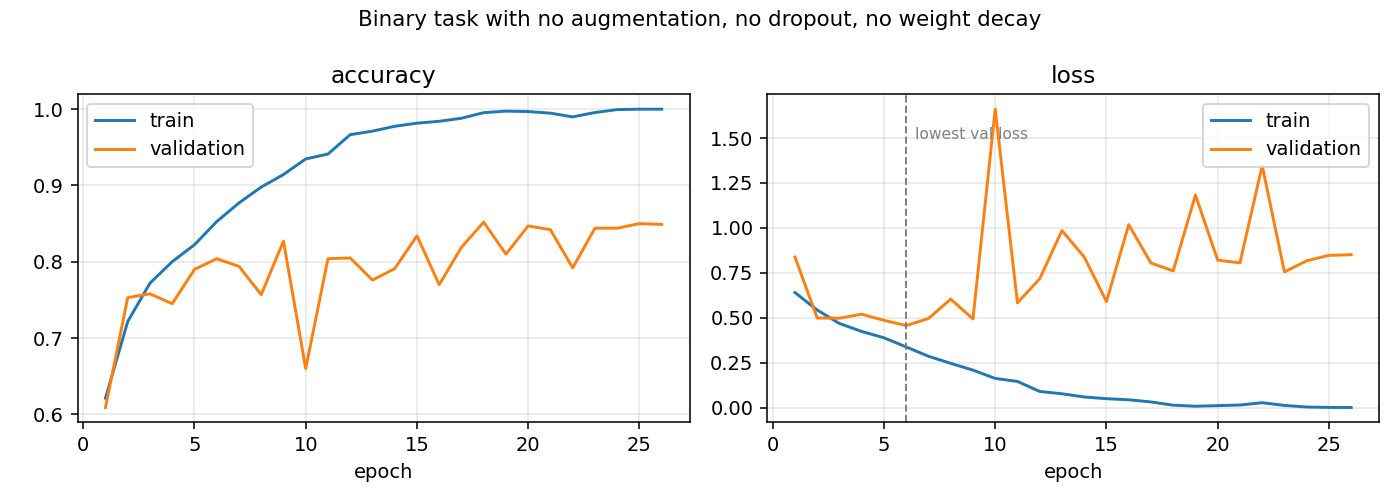
\includegraphics[width=0.95\textwidth]{cls_overfit_curves.png}
\caption{The overfitting run. Training accuracy goes to 100\% while validation
accuracy stops improving, and validation loss turns upward after epoch 6 even
though training loss keeps falling: the model is memorising the training set.}
\end{figure}

\subsection{Explainability with Grad-CAM}

Grad-CAM shows which part of the image the network used for its decision. For a
predicted class $c$ with score $y^c$ and the feature maps $A^k$ of the last
convolutional layer, each map gets a weight equal to its average gradient, and
the heat map is the weighted sum passed through a ReLU:
\[
\alpha_k^c = \frac{1}{Z}\sum_{i,j}\frac{\partial y^c}{\partial A^k_{ij}},
\qquad
L^c = \mathrm{ReLU}\Big(\sum_k \alpha_k^c A^k\Big).
\]
The $4\times4$ map is upsampled to $32\times32$ and drawn over the image. I made
one figure for correct predictions and one for mistakes. On correct predictions
the heat is mostly on the animal. On several mistakes it is on the background,
which explains why the network was wrong.

\begin{figure}[H]
\centering
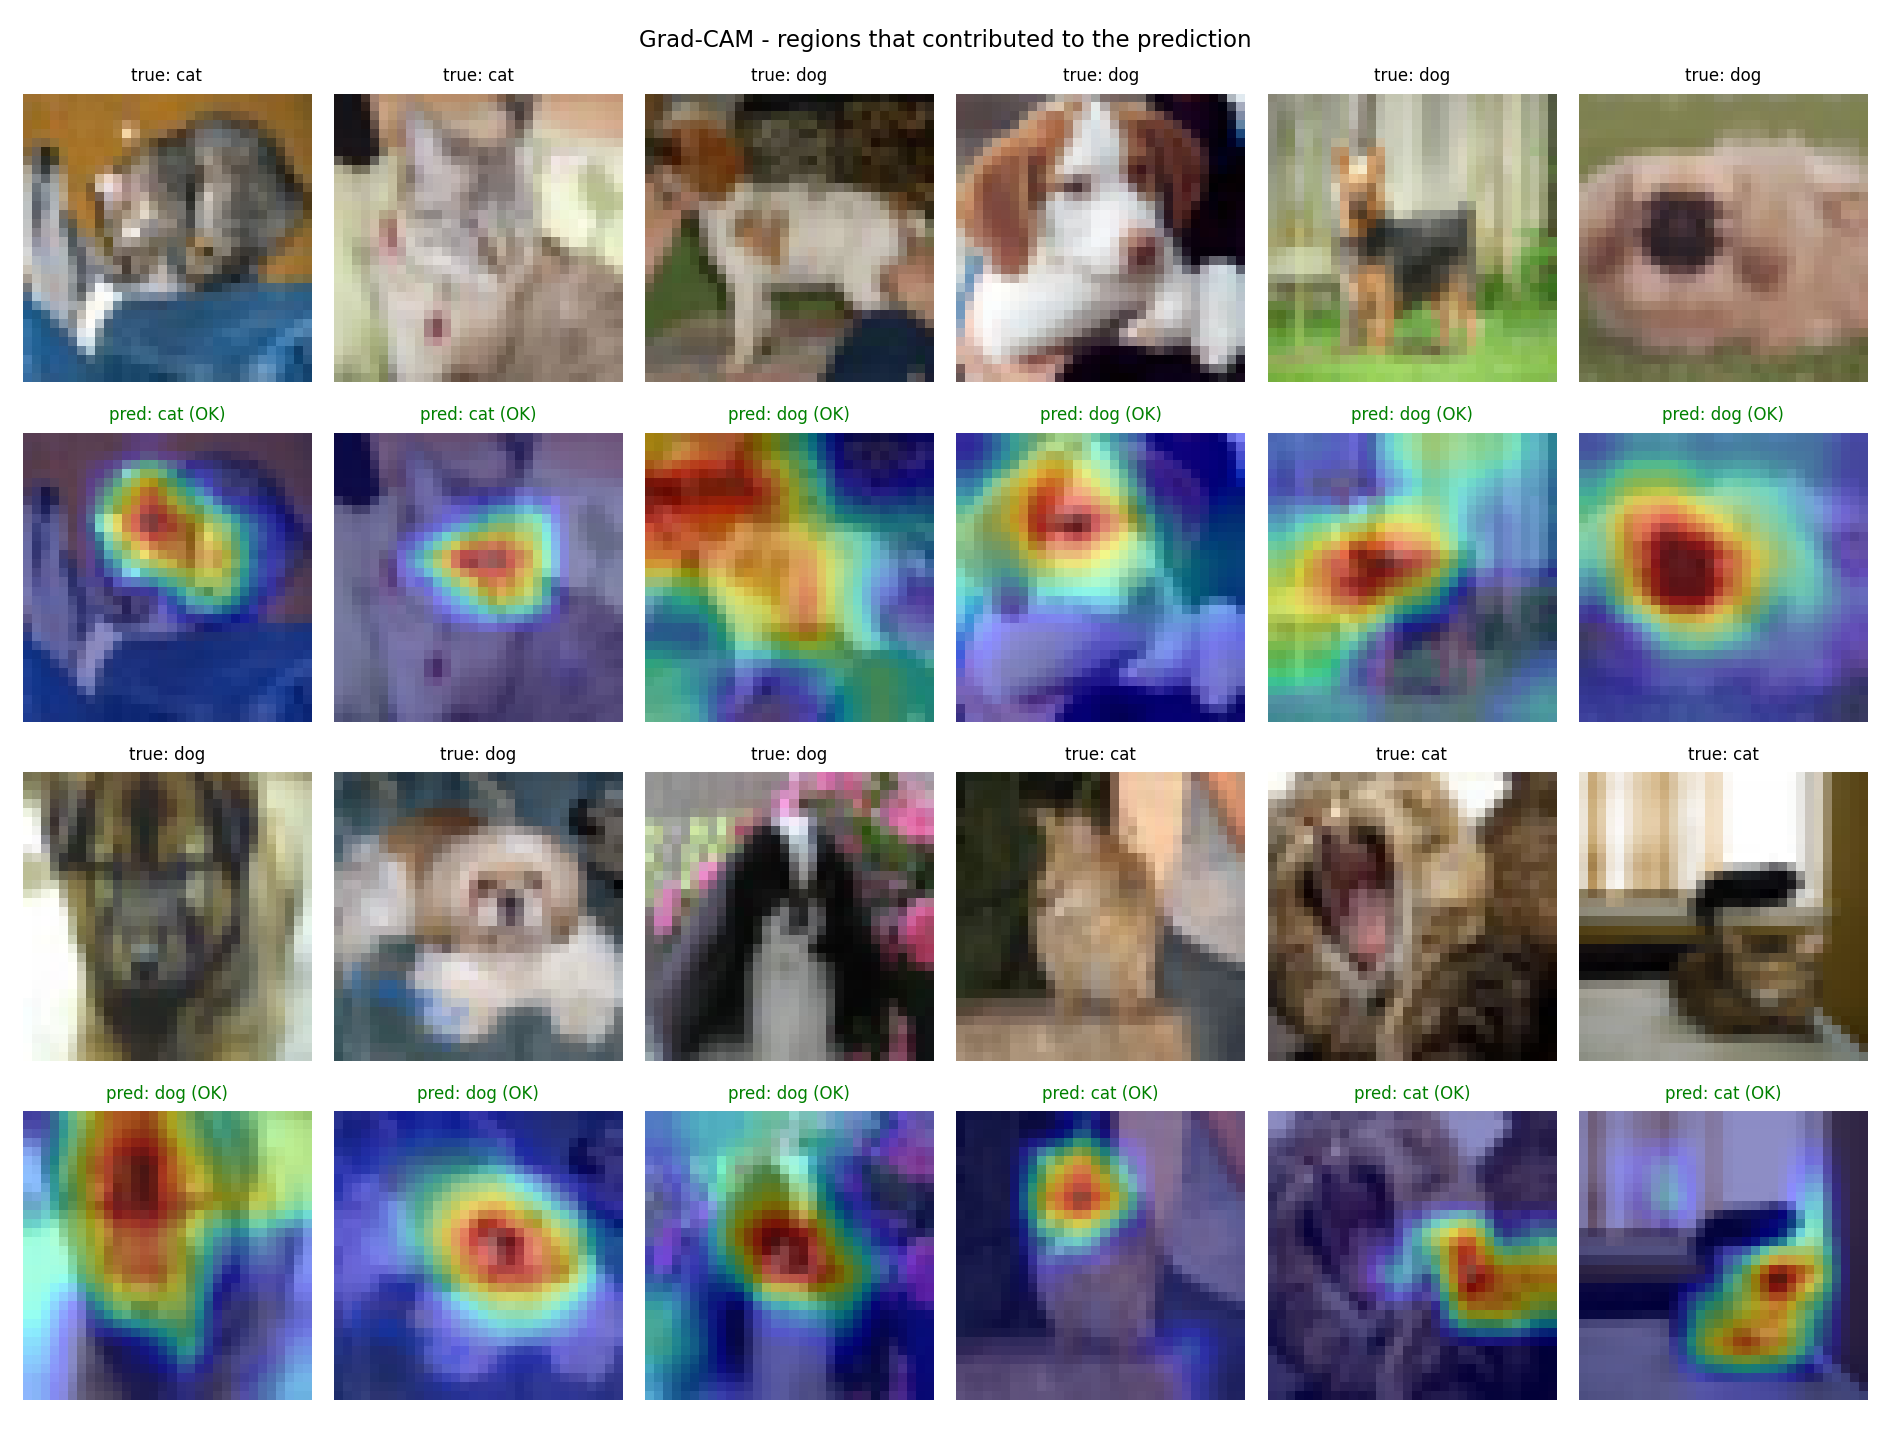
\includegraphics[width=0.48\textwidth]{cls_gradcam_correct.png}\hfill
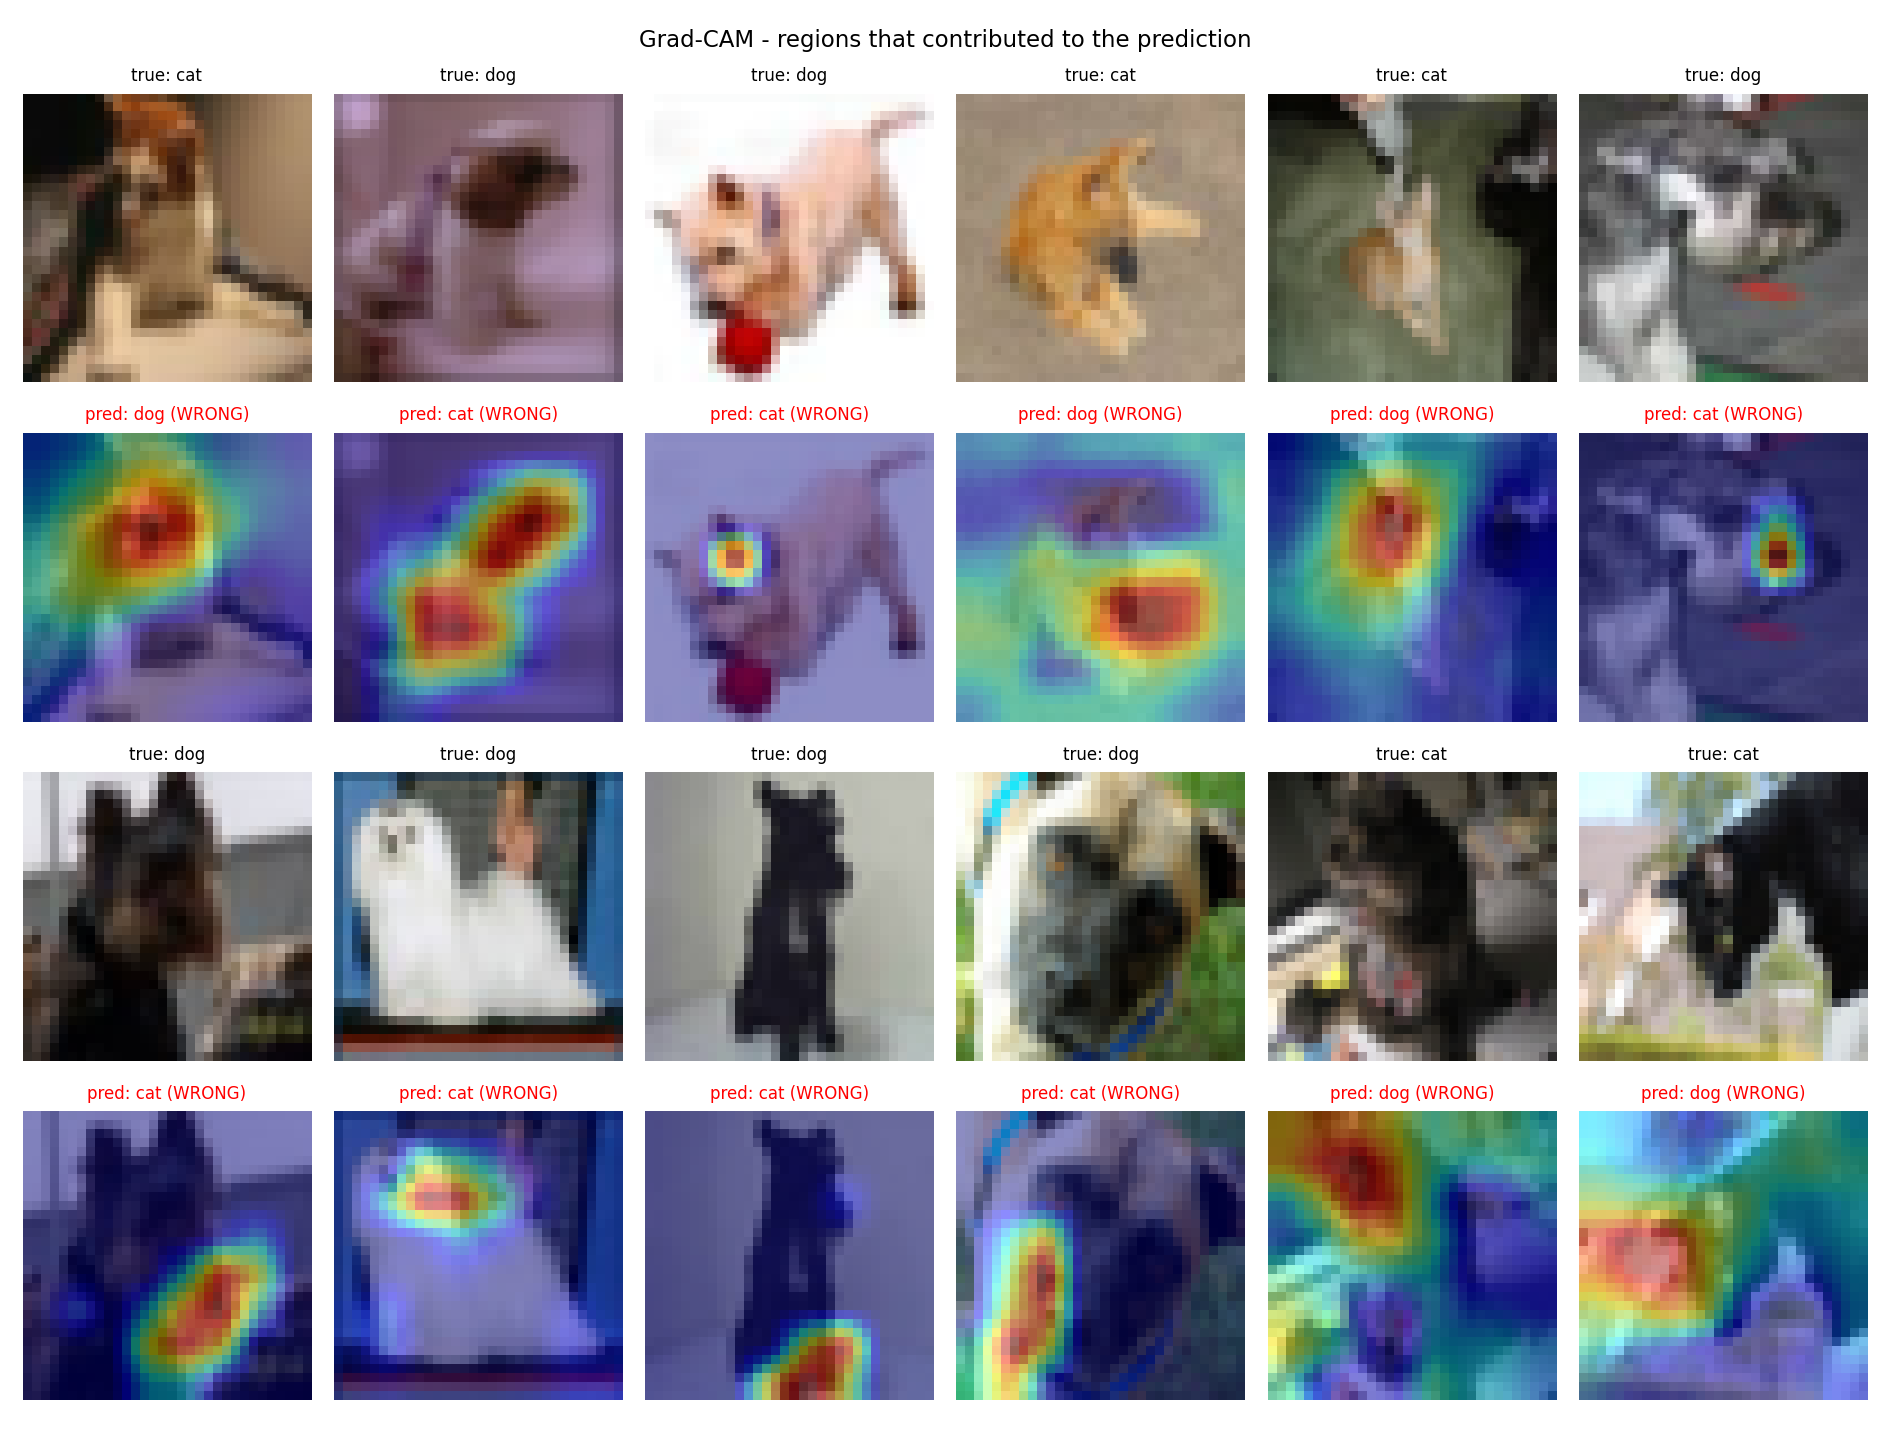
\includegraphics[width=0.48\textwidth]{cls_gradcam_errors.png}
\caption{Grad-CAM on correct predictions (left) and on mistakes (right).}
\end{figure}

% =====================================================================
\section{Project 2: liver and tumour segmentation}\label{sec:seg}
% =====================================================================

\subsection{Problem}

Given one axial CT slice of the abdomen, label every pixel as background, liver
or tumour. Radiologists outline the liver and each lesion by hand across hundreds
of slices per patient, which is slow and differs between readers. An automatic
segmentation is the first step towards measuring liver and tumour volume.

\subsection{Dataset}

I used LiTS, the Liver Tumor Segmentation Benchmark, in a version exported as 2D
PNG slices. Before writing any training code I wrote a script that only reads the
dataset and describes it (\code{dataset\_report.py}).

\begin{table}[H]
\centering\small
\begin{tabular}{lll}
\toprule
\textbf{Property} & \textbf{Value} & \textbf{Consequence} \\
\midrule
patients & 131 & split by patient \\
slices & 58{,}638, $256\times256$, 8-bit & \\
slices per patient & 74 to 987 & slice thickness differs a lot \\
slices with no liver & 67.4\% & dropped from training \\
usable slices & 19{,}143 & \\
background pixels & 97.74\% & accuracy is meaningless \\
liver pixels & 2.15\% & \\
tumour pixels & 0.12\% & Dice-based loss \\
masks & 2 binary PNGs per slice & merged, lesion written last \\
\bottomrule
\end{tabular}
\caption{Dataset properties and the design decision each one forced.}
\label{tab:seg_data}
\end{table}

\paragraph{The first version had damaged labels.} The first copy of the dataset
I downloaded stored the masks as JPEG. JPEG is lossy: it is fine for photographs
but wrong for label images, where the pixel value \emph{is} the class. The dataset
report found pixel values that are not valid classes, including a value that maps
to class 3 in a three-class problem. This proved that compression had changed the
labels, so I switched to a lossless PNG export of the same data.

\paragraph{Merging the two masks.} In the PNG version each slice has two binary
masks: one for the liver and one for the lesion. They are merged into one mask
with values 0, 1, 2. The liver mask also covers the lesion, so the lesion must be
written \emph{last}:
\[
y = \mathbb{1}[\text{liver} > 0], \qquad y[\text{lesion} > 0] = 2 .
\]
In the other order every tumour pixel is overwritten with liver and the tumour
class disappears from the data, with no error message. A check confirmed that
100\% of lesion pixels lie inside the liver mask.

\paragraph{Incomplete download guard.} On one machine the download was
interrupted and only 31{,}871 of the 58{,}638 slices had a liver mask. The code
ran without errors and produced plausible but wrong results on a much smaller
test set. The loader now refuses to start if the number of images does not match
the number of complete (image, liver mask, lesion mask) triples.

\subsection{Data pipeline}

\paragraph{Patient-level split.} My first version split individual slices at
random. That is wrong for this data: neighbouring slices of the same patient are a
few millimetres apart and nearly identical, so a random split puts almost the same
image into both training and test. The score then measures memorisation. The
final version shuffles the 131 \emph{patients} with a fixed seed and assigns whole
patients to each set, 15\% for test and 15\% for validation.

\begin{table}[H]
\centering\small
\begin{tabular}{lrr}
\toprule
\textbf{Set} & \textbf{Patients} & \textbf{Slices with liver} \\
\midrule
train & 91 & 13{,}745 \\
validation & 20 & 3{,}151 \\
test & 20 & 2{,}247 \\
\bottomrule
\end{tabular}
\caption{Patient-level split, seed 42.}
\end{table}

\paragraph{Empty slices.} Slices whose ground truth contains no liver are
dropped (\code{skip\_empty}). Training on them mostly teaches the network to answer
``background''. The same rule is used for validation and test, so all reported
numbers are on slices that contain liver.

\paragraph{Preprocessing.} Images are scaled to $[0,1]$ and normalised as
$x' = (x - 0.5)/0.5$. Images are resized with bilinear interpolation, but masks
are always resized with \emph{nearest neighbour}: interpolating between class 1
and class 2 would invent a class 1.5.

\paragraph{Augmentation.} Random horizontal flip, random vertical flip and a
random rotation by 0, 90, 180 or 270 degrees, each applied with the \emph{same}
parameters to the image and its mask. These transformations only move pixels, so
mask values stay exact integers.

\subsection{Architectures}

Both networks are built from the same four blocks, so the only difference between
them is the one being tested.

\begin{itemize}
  \item \code{DoubleConv}: two $3\times3$ convolutions, each with batch
        normalisation and ReLU.
  \item \code{Down}: $2\times2$ max pooling, then \code{DoubleConv}. Halves the
        resolution and doubles the channels.
  \item \code{Up}: a $2\times2$ transposed convolution that doubles the resolution
        and halves the channels, concatenation with the skip connection, then
        \code{DoubleConv}.
  \item \code{AttentionGate}: only in the Attention U-Net, described below.
\end{itemize}

\paragraph{U-Net.} The encoder applies four \code{Down} blocks, so the channels go
$32 \to 64 \to 128 \to 256 \to 512$ and a $256\times256$ slice becomes
$16\times16$ at the bottleneck. The decoder reverses this. At each level it
concatenates the encoder output of the same resolution (the skip connection),
which brings back the fine detail that pooling threw away. A final $1\times1$
convolution gives three scores per pixel.

\paragraph{Attention U-Net.} In a plain U-Net the skip connection passes
everything from the encoder to the decoder: liver, but also ribs, spine, kidneys
and bowel. The Attention U-Net filters each skip connection first. The gate takes
the skip features $x$ and a gating signal $g$, the coarser decoder features from
the level below, which carry more context about \emph{where} the organ is. Both
are projected to an intermediate size with $1\times1$ convolutions, $g$ is
upsampled to the size of $x$, and the result is a weight between 0 and 1 for every
pixel:
\[
\alpha = \sigma\!\left(\psi^{\top}\,\mathrm{ReLU}\!\left(W_g\, g + W_x\, x\right)\right),
\qquad \hat{x} = x \odot \alpha .
\]
The skip connection is multiplied by $\alpha$ before concatenation, so regions the
decoder considers irrelevant are suppressed.

\begin{table}[H]
\centering\small
\begin{tabular}{lrr}
\toprule
\textbf{Component} & \textbf{U-Net} & \textbf{Attention U-Net} \\
\midrule
input \code{DoubleConv} ($1\to32$) & 9{,}632 & 9{,}632 \\
encoder \code{Down} 1 to 3 ($32\to256$) & 1{,}163{,}008 & 1{,}163{,}008 \\
bottleneck \code{Down} 4 ($256\to512$) & 3{,}540{,}992 & 3{,}540{,}992 \\
decoder \code{Up} blocks & 3{,}048{,}800 & 3{,}048{,}800 \\
attention gates & -- & 132{,}252 \\
output $1\times1$ convolution & 99 & 99 \\
\midrule
\textbf{total} & \textbf{7{,}762{,}531} & \textbf{7{,}894{,}783} \\
\bottomrule
\end{tabular}
\caption{Parameter counts by component. The difference between the networks,
132{,}252 parameters (1.7\%), is exactly the four attention gates. These counts
were computed by hand from the layer sizes and checked against PyTorch's own count
and the generated diagram.}
\label{tab:seg_params}
\end{table}

Almost half of the parameters (45.6\%) are in the bottleneck block, because a
$3\times3$ convolution with 512 input and 512 output channels alone has 2.4
million weights. The four gates are small, and most of their size is in the
deepest one (99{,}203 parameters).

\begin{figure}[p]
\centering
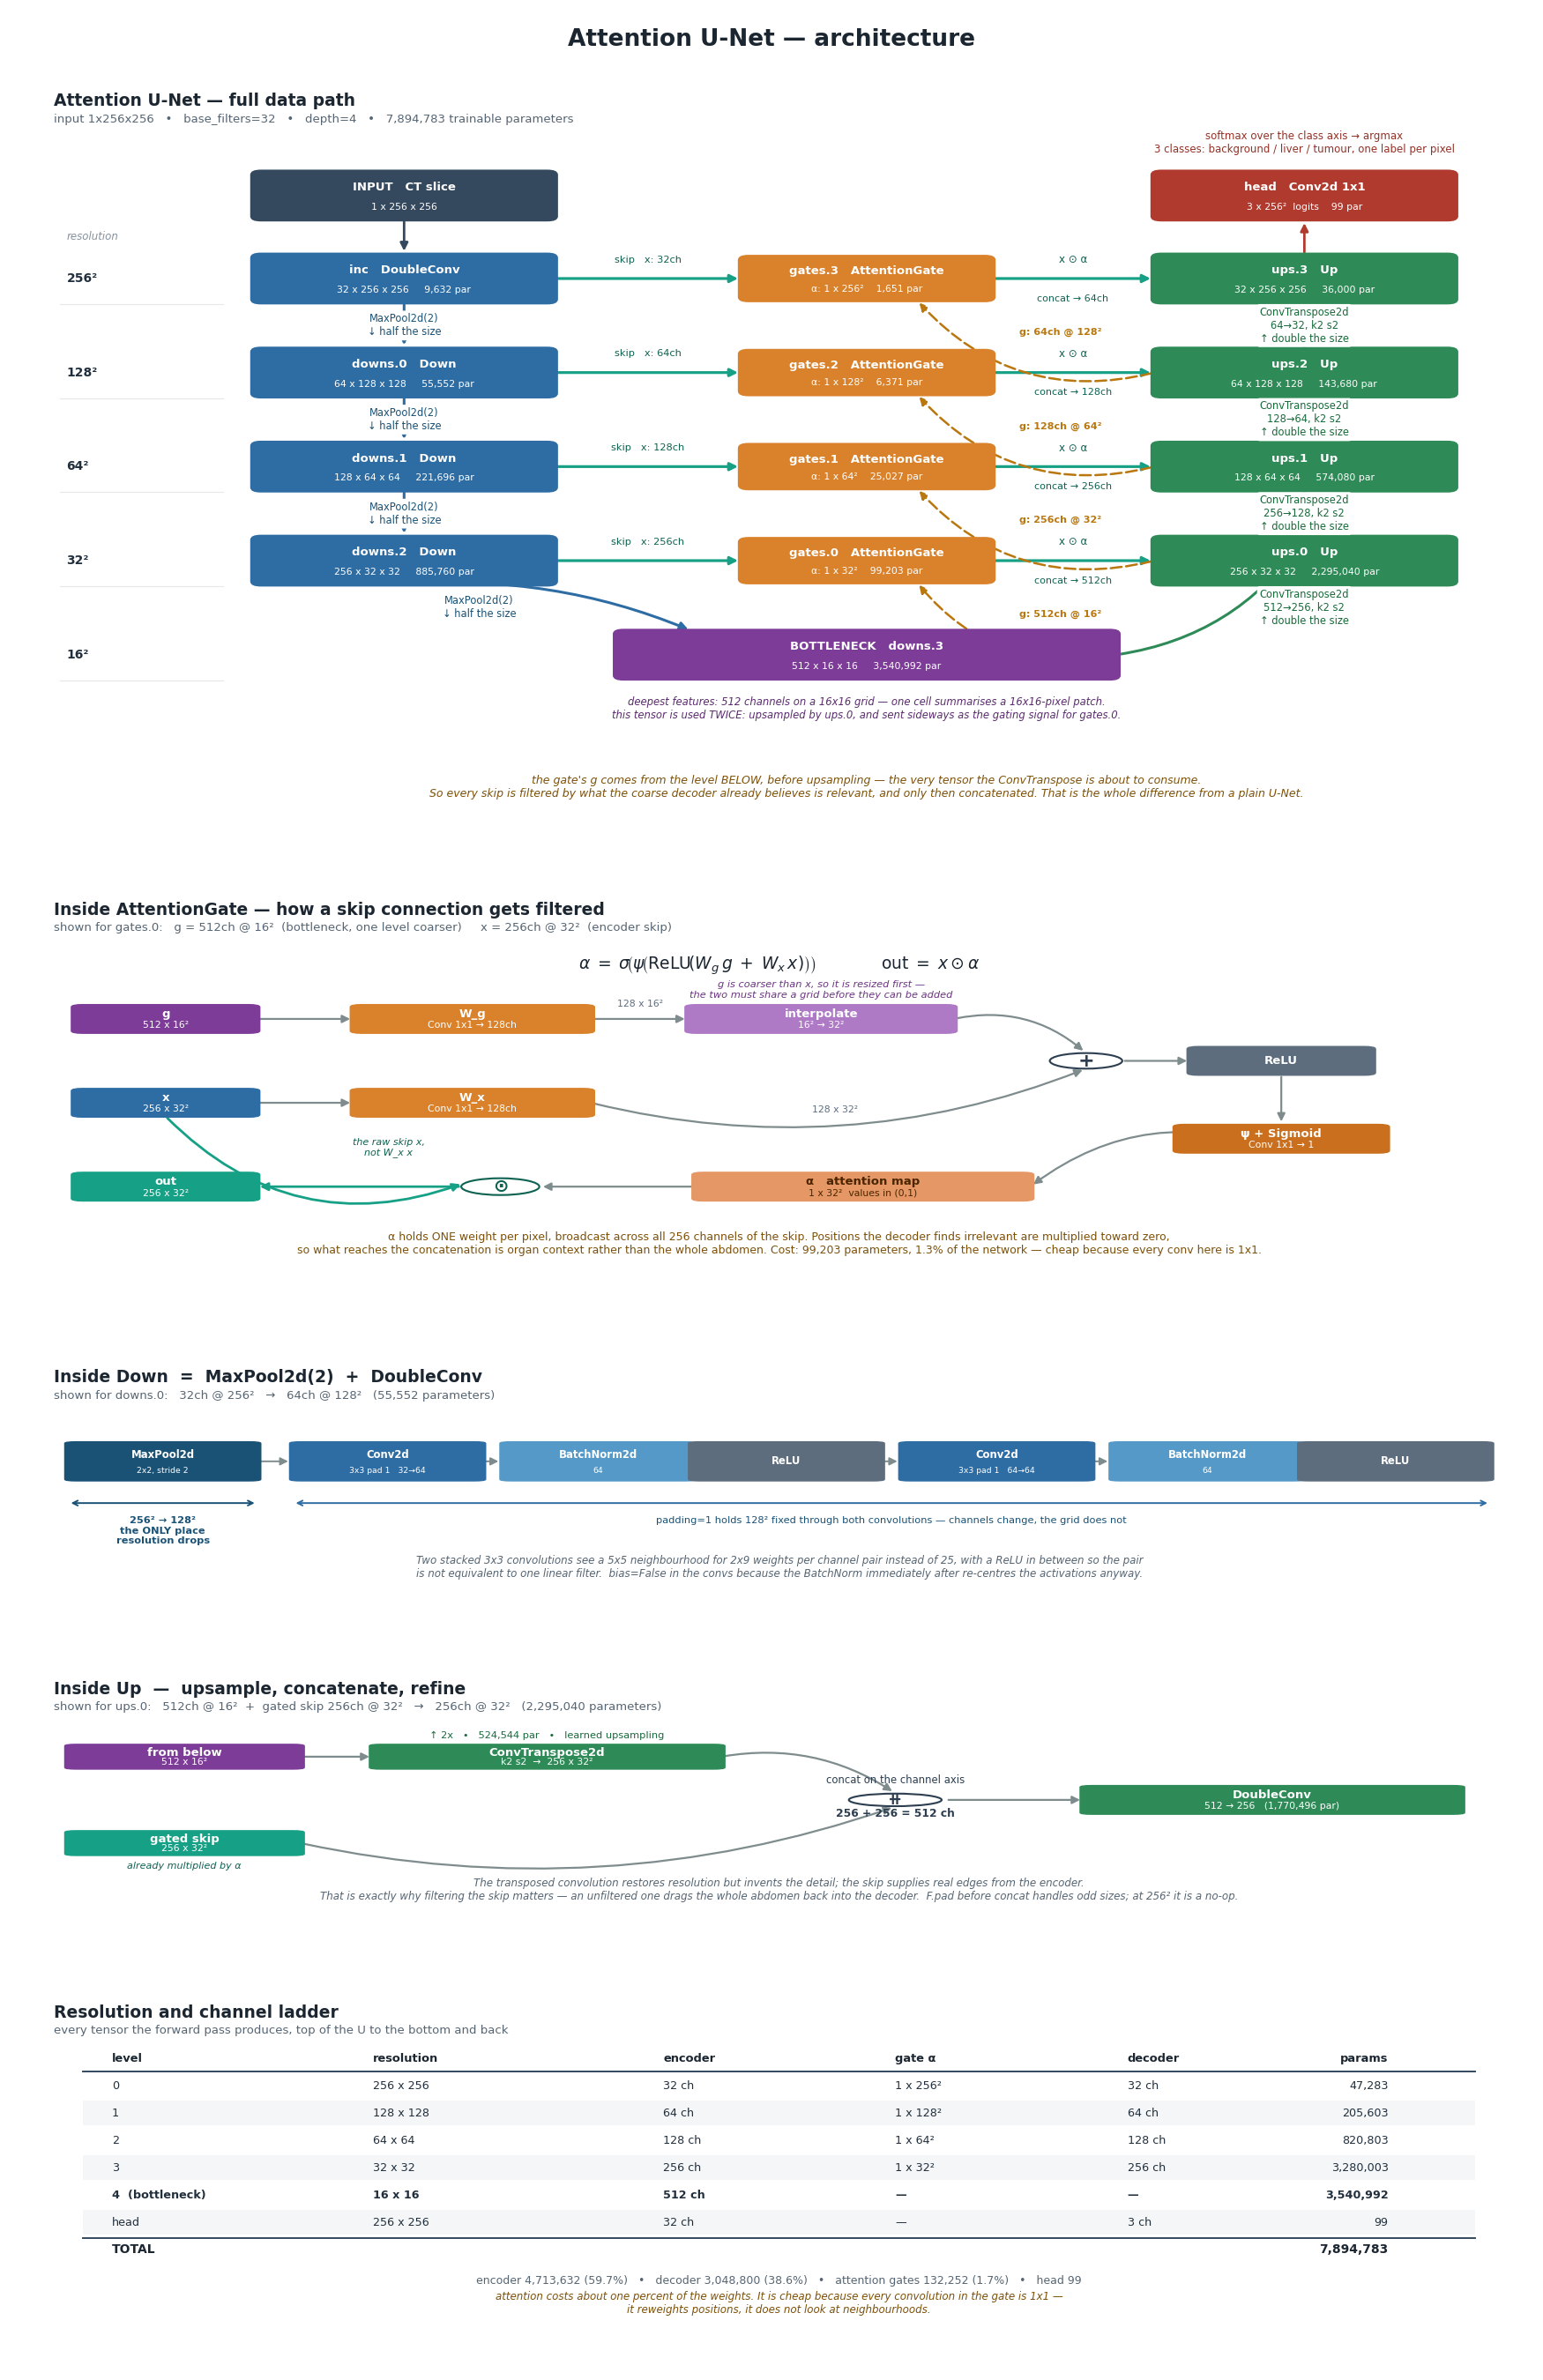
\includegraphics[height=0.86\textheight,keepaspectratio]{attention_unet_diagram.png}
\caption{The Attention U-Net, generated from the code so that shapes and
parameter counts cannot drift from the implementation. The gates sit on the skip
connections; the dashed arrows are the gating signals from the level below.}
\end{figure}

\subsection{Loss function}

Plain cross-entropy is dominated by background, which is 97.7\% of the pixels: a
network can get a low loss while ignoring the tumour. I combined it with a soft
Dice loss, which is computed per class and normalised by the size of that class,
so tumour counts as much as background. With softmax probabilities $p$, the
one-hot ground truth $t$, and the sum over all pixels of the batch:
\[
\mathcal{L}_{\text{Dice}} = 1 - \frac{1}{C}\sum_{c=1}^{C}
\frac{2\sum_i p_{i,c}\, t_{i,c} + \varepsilon}{\sum_i p_{i,c} + \sum_i t_{i,c} + \varepsilon},
\qquad
\mathcal{L} = 0.5\,\mathcal{L}_{\text{Dice}} + 0.5\,\mathcal{L}_{\text{CE}},
\]
with $\varepsilon = 1$ to avoid division by zero when a class is missing from a
batch. Optional class weights for the cross-entropy term are implemented (inverse
frequency or manual) but were not used in the final runs.

\subsection{Evaluation metrics}

Everything is computed from one $3\times3$ confusion matrix accumulated over all
pixels of the test set. For each class:
\begin{align*}
\text{Dice} &= \frac{2\,TP}{2\,TP + FP + FN}, &
\text{IoU} &= \frac{TP}{TP + FP + FN},\\[4pt]
\text{precision} &= \frac{TP}{TP+FP}, &
\text{recall} &= \frac{TP}{TP+FN}.
\end{align*}
Dice is the F1 score applied to pixels. Dice and IoU always rank results the same
way, since $\text{IoU} = \text{Dice}/(2-\text{Dice})$.

\paragraph{Why not accuracy.} On the test slices, background is 93.42\% of the
pixels. A model that predicts background everywhere scores 93.4\% pixel accuracy
and segments nothing. The trained model scores 98.9\%. That looks like a small
gain, but foreground Dice goes from 0.000 to 0.825. For this reason the best epoch
is chosen by the \textbf{mean foreground Dice}, the average Dice of liver and
tumour only, on the validation set. Accuracy and loss are never used to select a
model.

\subsection{Training setup}

\begin{table}[H]
\centering\small
\begin{tabular}{ll}
\toprule
\textbf{Setting} & \textbf{Value} \\
\midrule
input & 1 channel, $256\times256$ \\
loss & $0.5\,$Dice $+\,0.5\,$cross-entropy \\
optimiser & Adam, learning rate $10^{-3}$, weight decay $10^{-4}$ \\
schedule & cosine annealing over 40 epochs \\
batch size & 8 \\
precision & mixed (float16 forward pass with gradient scaling) \\
initialisation & Kaiming for convolutions, BN weight 1 and bias 0 \\
dropout & none \\
early stopping & disabled (see Section~\ref{sec:seg_invalid}) \\
model selection & best validation foreground Dice \\
seed & 42, the same for both architectures \\
\bottomrule
\end{tabular}
\caption{Segmentation training setup, identical for both networks.}
\end{table}

The training history is written to disk after every epoch, and stopping the
run with Ctrl+C keeps the best checkpoint and evaluates it, so a long run is never
lost because of an interruption.

\subsection{A first comparison that was not valid}\label{sec:seg_invalid}

The first comparison ran on the laptop with early stopping enabled (patience 10
epochs). The results suggested a clear winner:

\begin{table}[H]
\centering\small
\begin{tabular}{lrrrr}
\toprule
\textbf{Model} & \textbf{Epochs run} & \textbf{Best epoch} & \textbf{Test fg Dice} & \textbf{Tumour Dice} \\
\midrule
U-Net           & 40 & 32 & 0.8191 & 0.7334 \\
Attention U-Net & 28 & 18 & 0.7633 & 0.6400 \\
\bottomrule
\end{tabular}
\caption{The first, invalid comparison (laptop, early stopping on).}
\end{table}

A gap of 0.056 looked like a real result, but the two models had not been
trained for the same time. The Attention U-Net's validation score plateaued
early, early stopping ended it at epoch 28, and the U-Net got 12 more epochs at
the low end of the cosine schedule. The comparison measured the training budget,
not the architecture. I disabled early stopping by default and retrained both for
the full 40 epochs. The gap disappeared (Table~\ref{tab:seg_results}).

\subsection{Results}

\begin{table}[H]
\centering\small
\setlength{\tabcolsep}{4.5pt}
\begin{tabular}{lrrrrrr}
\toprule
\textbf{Model} & \textbf{Val fg Dice} & \textbf{Test fg Dice} & \textbf{fg IoU}
& \textbf{Liver} & \textbf{Tumour} & \textbf{Time} \\
\midrule
U-Net           & \textbf{0.8550} & 0.8222 & 0.7076 & 0.9101 & \textbf{0.7343} & 93 min \\
Attention U-Net & 0.8432 & \textbf{0.8247} & \textbf{0.7123} & \textbf{0.9172} & 0.7322 & 112 min \\
\bottomrule
\end{tabular}
\caption{Final results, RTX 2070, 40 epochs each, same split and seed, test set
of 2{,}247 slices from 20 patients. Best validation epoch: 40 for U-Net, 37 for
Attention U-Net.}
\label{tab:seg_results}
\end{table}

\begin{table}[H]
\centering\small
\begin{tabular}{llrrrr}
\toprule
\textbf{Model} & \textbf{Class} & \textbf{Dice} & \textbf{IoU} & \textbf{Precision} & \textbf{Recall} \\
\midrule
U-Net & liver  & 0.9101 & 0.8350 & 0.9000 & 0.9205 \\
      & tumour & 0.7343 & 0.5802 & 0.8201 & 0.6648 \\
\midrule
Attention U-Net & liver  & 0.9172 & 0.8470 & 0.9106 & 0.9238 \\
                & tumour & 0.7322 & 0.5775 & 0.8163 & 0.6638 \\
\bottomrule
\end{tabular}
\caption{Per-class results on the test set.}
\end{table}

\begin{table}[H]
\centering\small
\begin{tabular}{lrrr}
\toprule
\textbf{True $\backslash$ predicted} & \textbf{background} & \textbf{liver} & \textbf{tumour} \\
\midrule
background & 136{,}801{,}462 & 757{,}191 & 11{,}244 \\
liver      & 638{,}000 & 8{,}493{,}783 & 62{,}699 \\
tumour     & 90{,}024 & 76{,}399 & 328{,}590 \\
\bottomrule
\end{tabular}
\caption{Pixel confusion matrix of the Attention U-Net on the test set. Every
metric above can be recomputed from these nine numbers.}
\label{tab:seg_cm}
\end{table}

\begin{figure}[H]
\centering
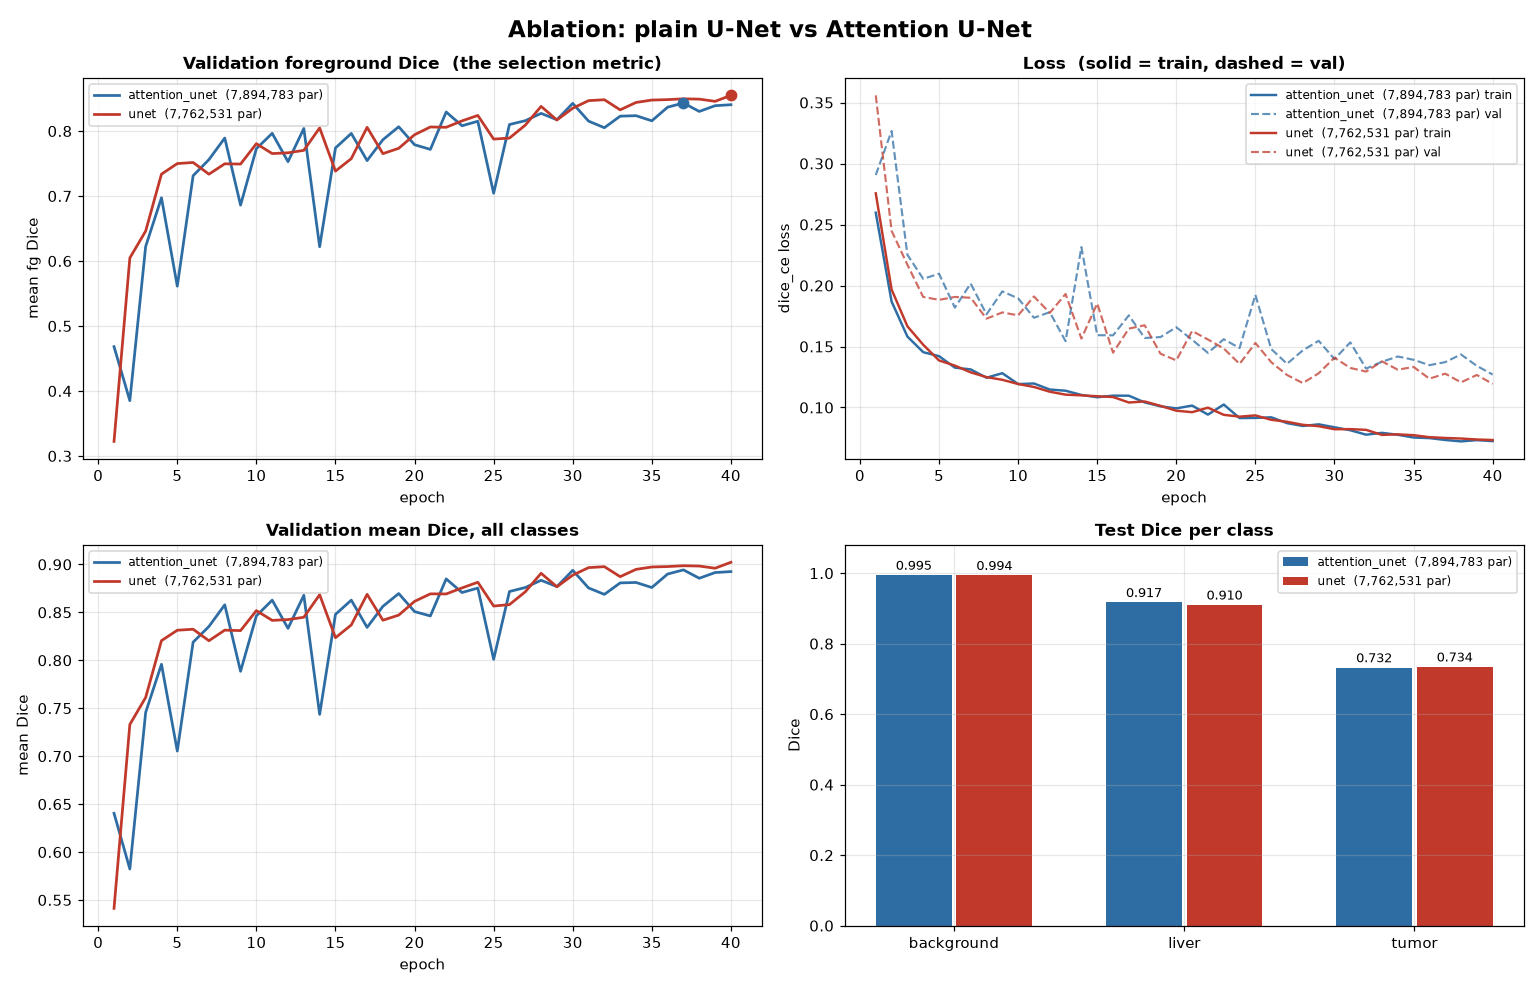
\includegraphics[width=\textwidth]{comparison_ablation.png}
\caption{Comparison of the two models: validation foreground Dice (used to pick
the best epoch), loss curves and test Dice per class.}
\end{figure}

\subsection{Analysis}

\paragraph{The architectures are not meaningfully different.} The Attention
U-Net is 0.0025 higher on foreground Dice and 0.0071 higher on liver, but 0.0021
lower on tumour. On the \emph{validation} set the order is reversed: the U-Net is
higher by 0.0118. When the sign of a difference depends on which set or which
class you look at, it is noise. The same U-Net configuration trained on the two
machines gave 0.8191 and 0.8222, a difference of 0.0031 from the hardware and
non-deterministic GPU operations alone. With one run per architecture, anything
below about 0.02 cannot be separated from run-to-run variation. The Attention
U-Net also took 20\% longer to train.

\paragraph{The real difficulty is the tumour.} Tumour precision is 0.816 but
recall only 0.664: when the model says tumour it is usually right, but it misses a
third of the actual tumour pixels. The confusion matrix shows where they go:
18.2\% of tumour pixels are predicted as background and 15.4\% as liver. Of the
582 test slices that contain a real lesion, 154 (26\%) have a tumour Dice of
exactly zero, meaning the lesion was missed completely on that slice. For a
screening tool this is the wrong direction to make mistakes in; one would rather
flag too much and let a radiologist dismiss it.

\begin{figure}[H]
\centering
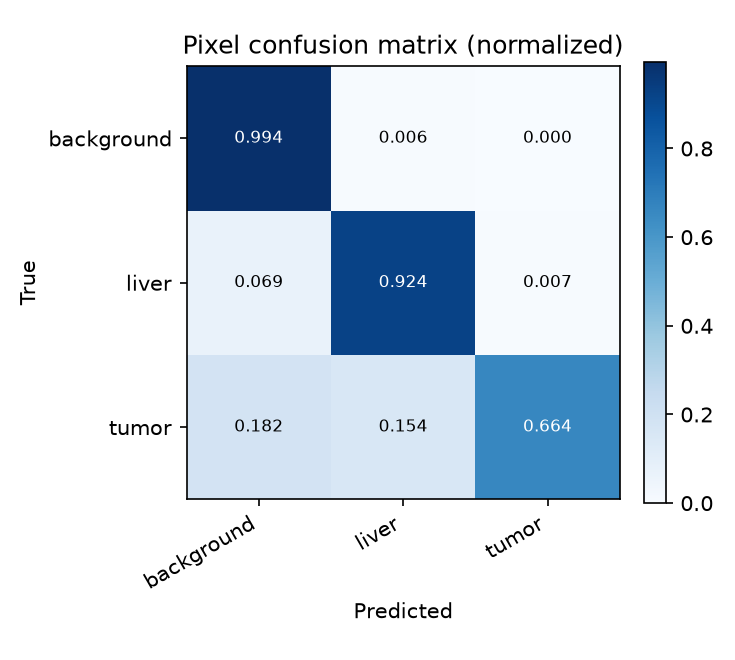
\includegraphics[width=0.50\textwidth]{attention_unet_confusion_test.png}\hfill
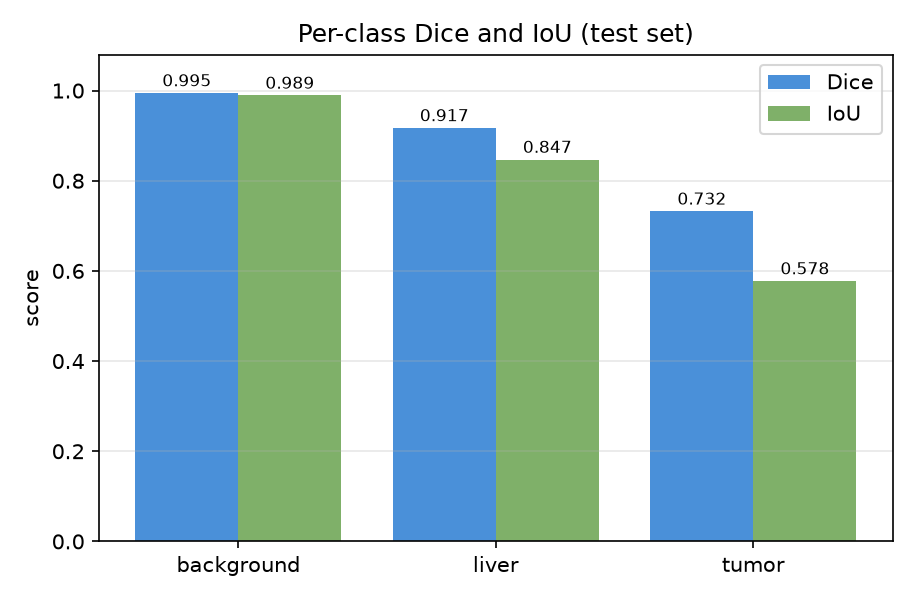
\includegraphics[width=0.48\textwidth]{attention_unet_dice_iou_test.png}
\caption{Attention U-Net on the test set. Left: confusion matrix normalised by
row (true class). Right: Dice and IoU per class.}
\end{figure}

\begin{figure}[H]
\centering
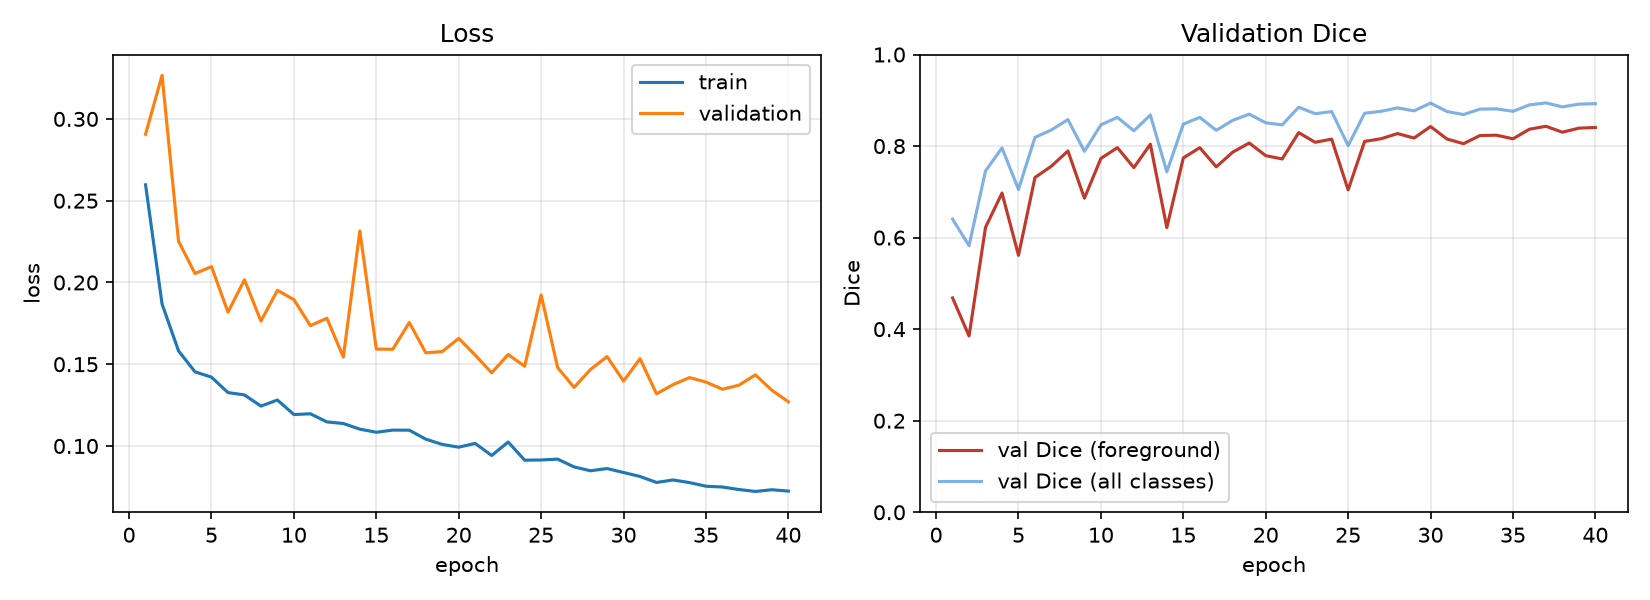
\includegraphics[width=0.85\textwidth]{attention_unet_training_curves.png}
\caption{Training curves of the Attention U-Net. Training loss falls steadily;
validation loss falls much more slowly, so the gap between them grows. The best
validation foreground Dice was at epoch 37.}
\end{figure}

\begin{figure}[p]
\centering
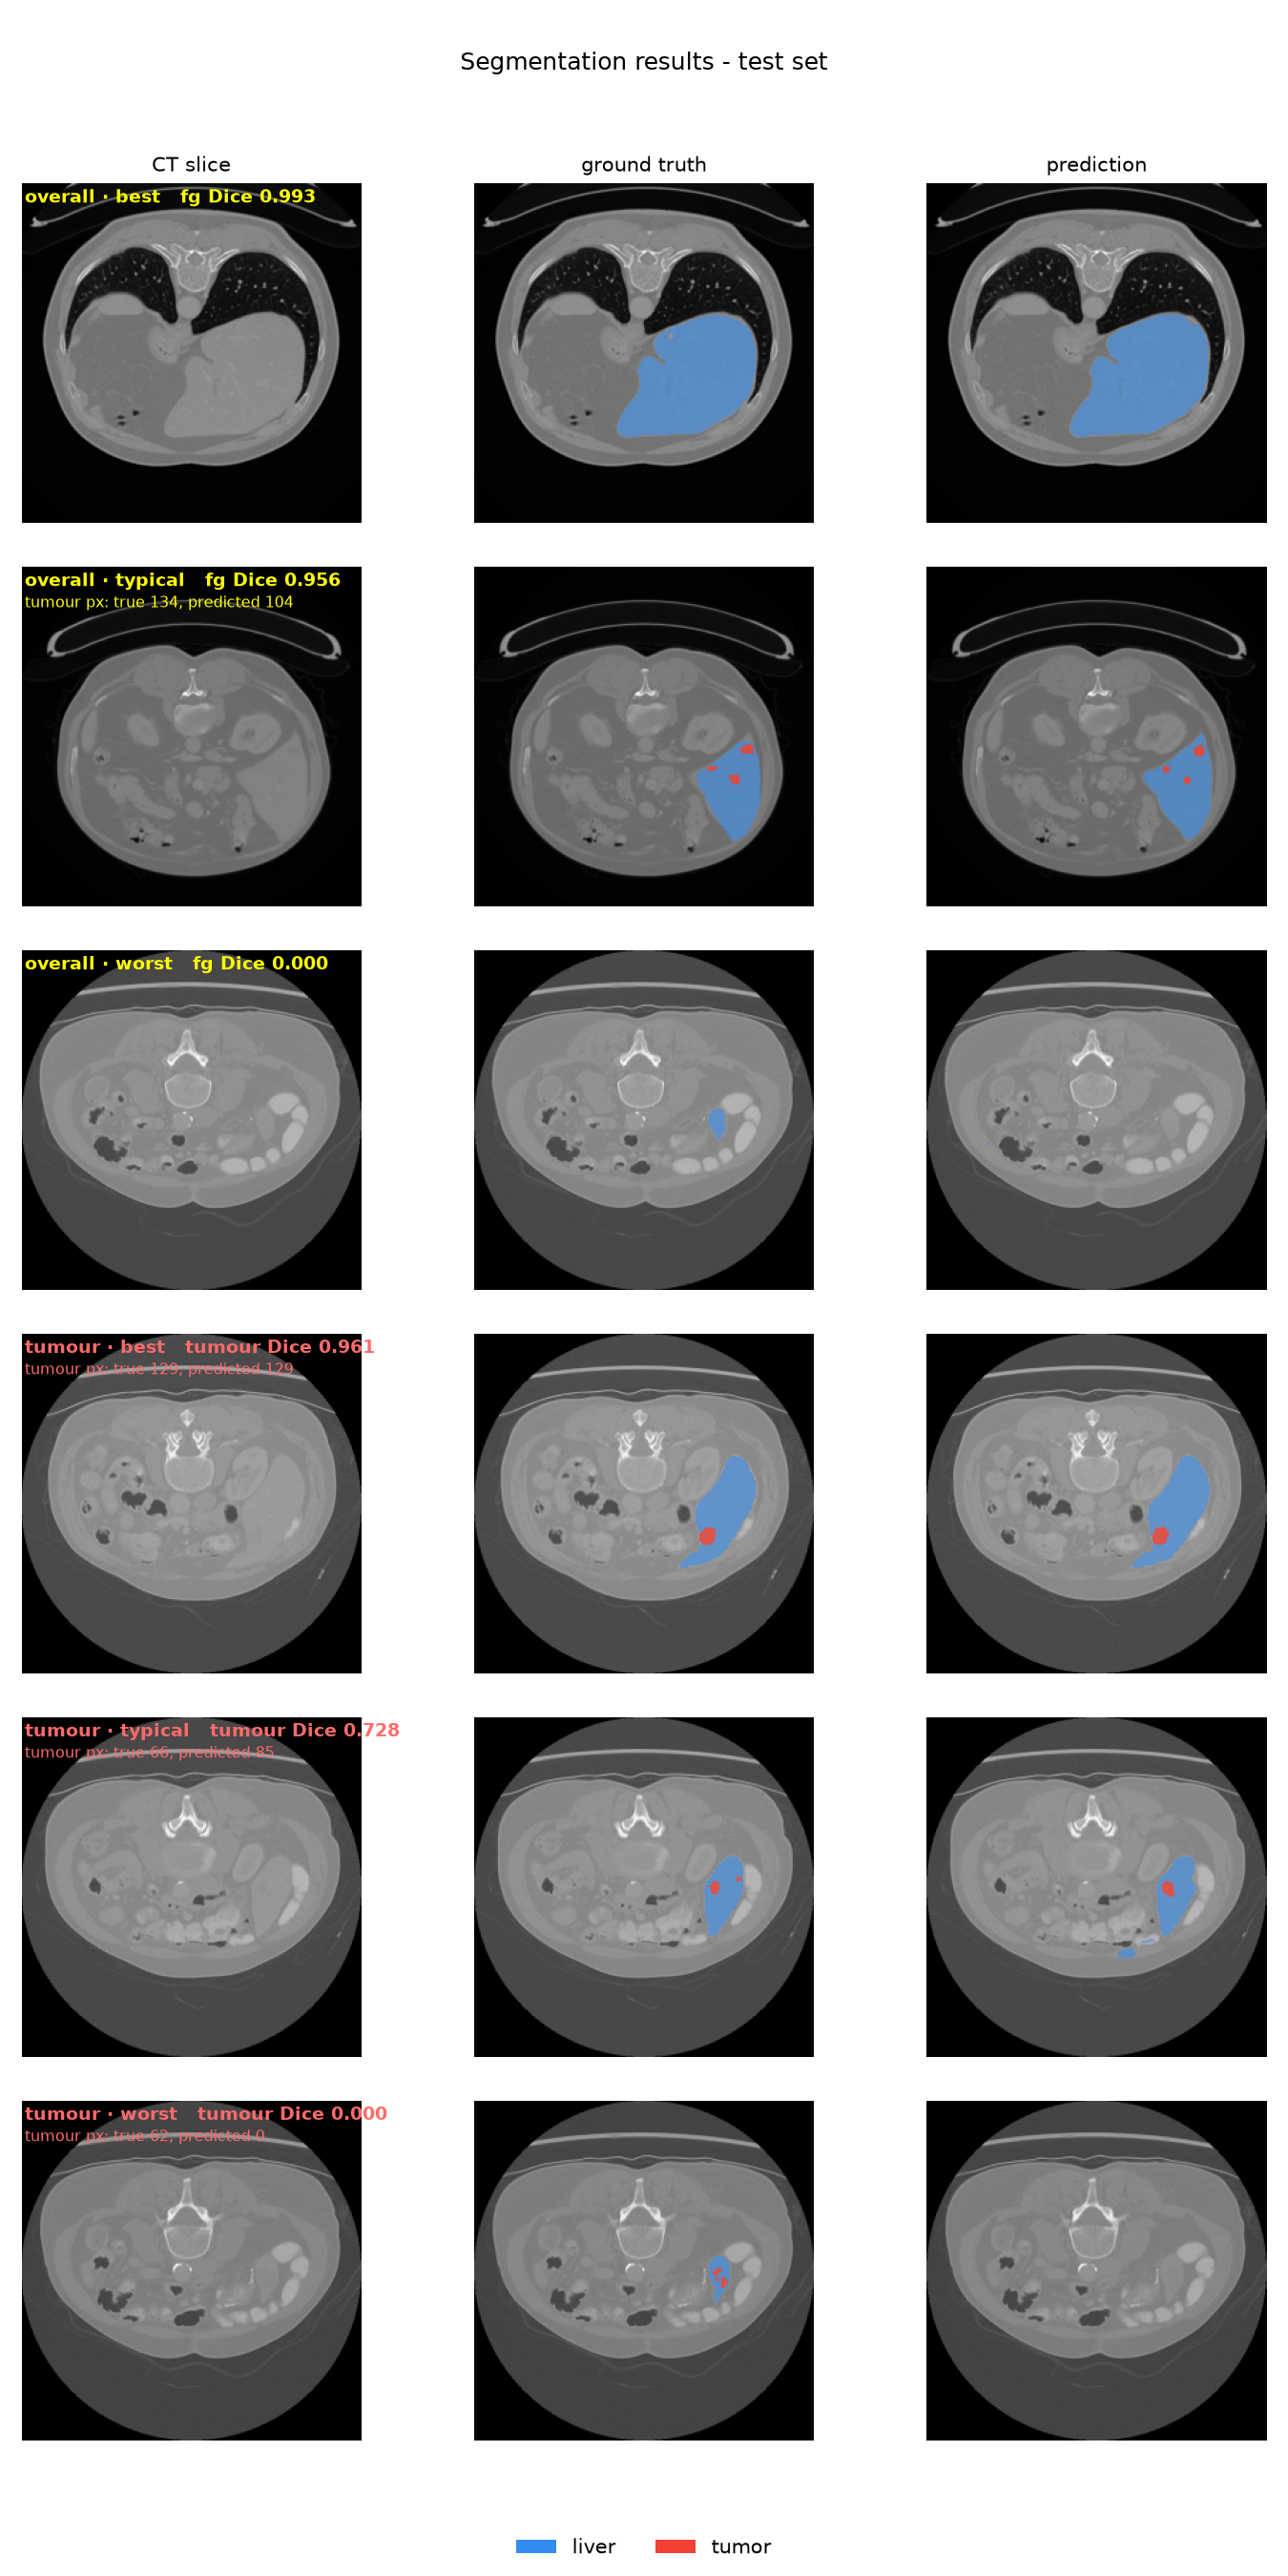
\includegraphics[height=0.86\textheight,keepaspectratio]{attention_unet_predictions_test.png}
\caption{Test predictions of the Attention U-Net: CT slice, ground truth and
prediction. The first rows are the best, a typical and the worst slice by
foreground Dice; the last rows are chosen the same way among slices with at least
50 tumour pixels, so the failures are shown as well as the successes.}
\end{figure}

\subsection{What the attention gates learned}

Since the gates did not improve the score, I checked whether they did anything
at all. A forward hook on the last layer of each gate records the $\alpha$ maps,
and I compared the mean $\alpha$ inside the ground-truth foreground with the mean
outside it, over many test slices.

The gates are selective: mean $\alpha$ inside the foreground is between 1.88 and
2.51 times higher than outside, depending on the gate, and the maps follow the
shape of the liver, becoming sharper at higher resolution. So the mechanism
works. One detail goes the wrong way: at the finest gate, the mean $\alpha$ on
tumour pixels is 0.327, against 0.760 inside the foreground as a whole. That gate
partly suppresses the tumour, the class the model already struggles with most.

My explanation for the lack of improvement is that the liver is large, has good
contrast and is always in roughly the same place in the abdomen, so the decoder
does not need help locating it. Dropping the 67\% of slices without liver already
removes much of the background the gates are meant to filter.

\subsection{3D reconstruction and visualisation}

The network segments one slice at a time and never sees the slices above or below.
Stacking the predictions back in scan order gives a 3D volume, and nothing in the
method forces the slices to join up into a plausible organ. To check this I wrote
two tools.

\paragraph{\code{view3d.py}: batch export.} For one patient it groups the
dataset files by patient, sorts them by the slice number in the file name (not
alphabetically, where \code{\_100} would come before \code{\_11}), keeps the
slices whose ground truth contains liver, runs the model on each slice and stacks
the CT, ground truth and prediction into three arrays of shape
$(n_{\text{slices}}, 256, 256)$. The arrays are preallocated as 8-bit integers;
building a list of float32 slices and stacking it used four times the memory and
crashed on a 689-slice patient. It writes PNG figures and, with \code{--nifti},
three \code{.nii.gz} files for 3D Slicer.

\paragraph{Voxel spacing.} The 2D export lost the original slice thickness, and a
viewer that assumes cubic voxels draws the patient badly stretched. The thickness
is estimated from the number of slices. The export is about 1.4\,mm per pixel and
an abdominal scan covers about 450\,mm, so the slice thickness in units of
in-plane pixels is
\[
z_{\text{scale}} \approx \frac{450 / n_{\text{slices}}}{1.4} \approx \frac{320}{n_{\text{slices}}} .
\]
For patient 16 (689 slices) this gives 0.464. The value is written into the NIfTI
affine as $\mathrm{diag}(1, 1, z_{\text{scale}}, 1)$, and the arrays are
transposed from $(z, y, x)$ to the $(x, y, z)$ order NIfTI expects. In 3D Slicer
the CT is loaded as a volume and the two label files as segmentations.

\paragraph{\code{viewer.py}: interactive viewer.} A window with axial, coronal
and sagittal views, an overlay of the ground truth, the prediction, or the
difference between them (correct, missed, false alarm), per-slice Dice, and a 3D
view that rotates when dragged. Two decisions in it were about speed, both found
by measuring. The first version was drawn with matplotlib, which redraws the whole
figure on every change, close to two million pixels per frame; the final version
uses \code{tkinter} widgets, so only the image is replaced, about eight times
less work per frame. And the 3D is not rendered live: marching cubes into a
matplotlib 3D axis took 4.7 seconds per redraw. Instead the volume is projected
ahead of time into 36 viewing angles with a depth buffer in \code{numpy}, about 2
seconds per overlay mode, and dragging just picks a precomputed frame.

\begin{figure}[H]
\centering
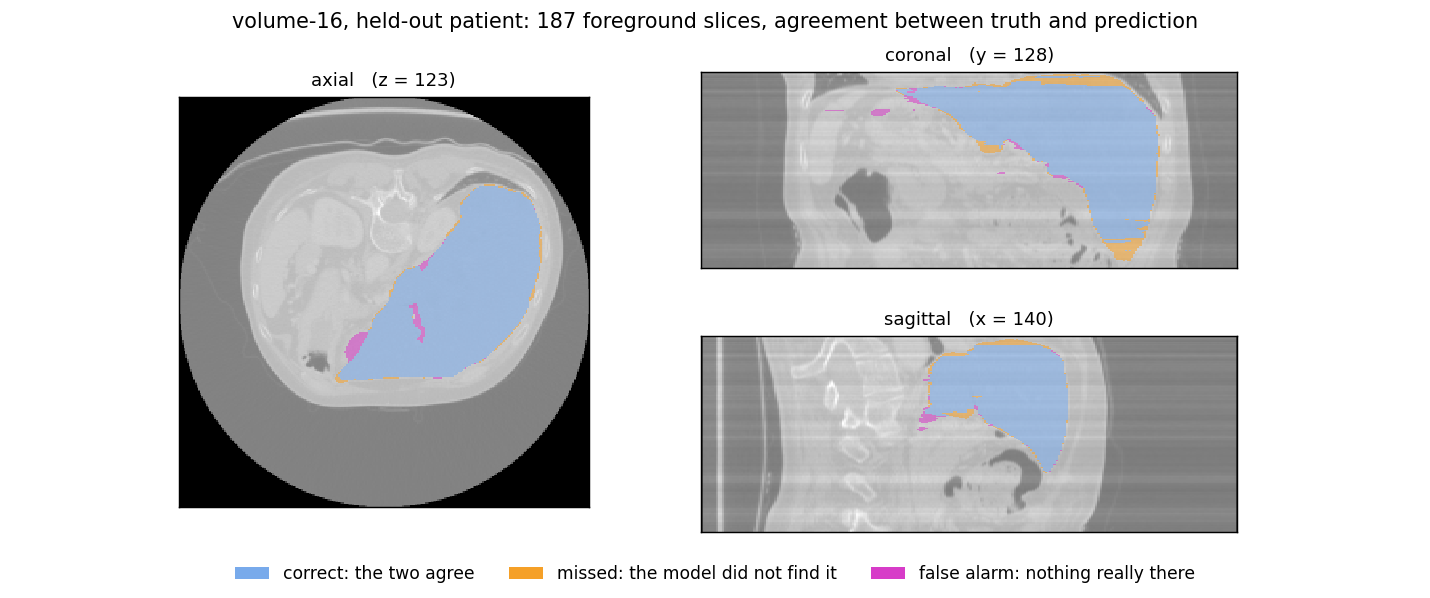
\includegraphics[width=\textwidth]{viewer_volume16_slices.png}
\caption{Patient 16 (held out), 187 slices with liver. The coronal and sagittal
views are rebuilt from the stack of 2D predictions; the network never saw them.}
\end{figure}

\begin{figure}[H]
\centering
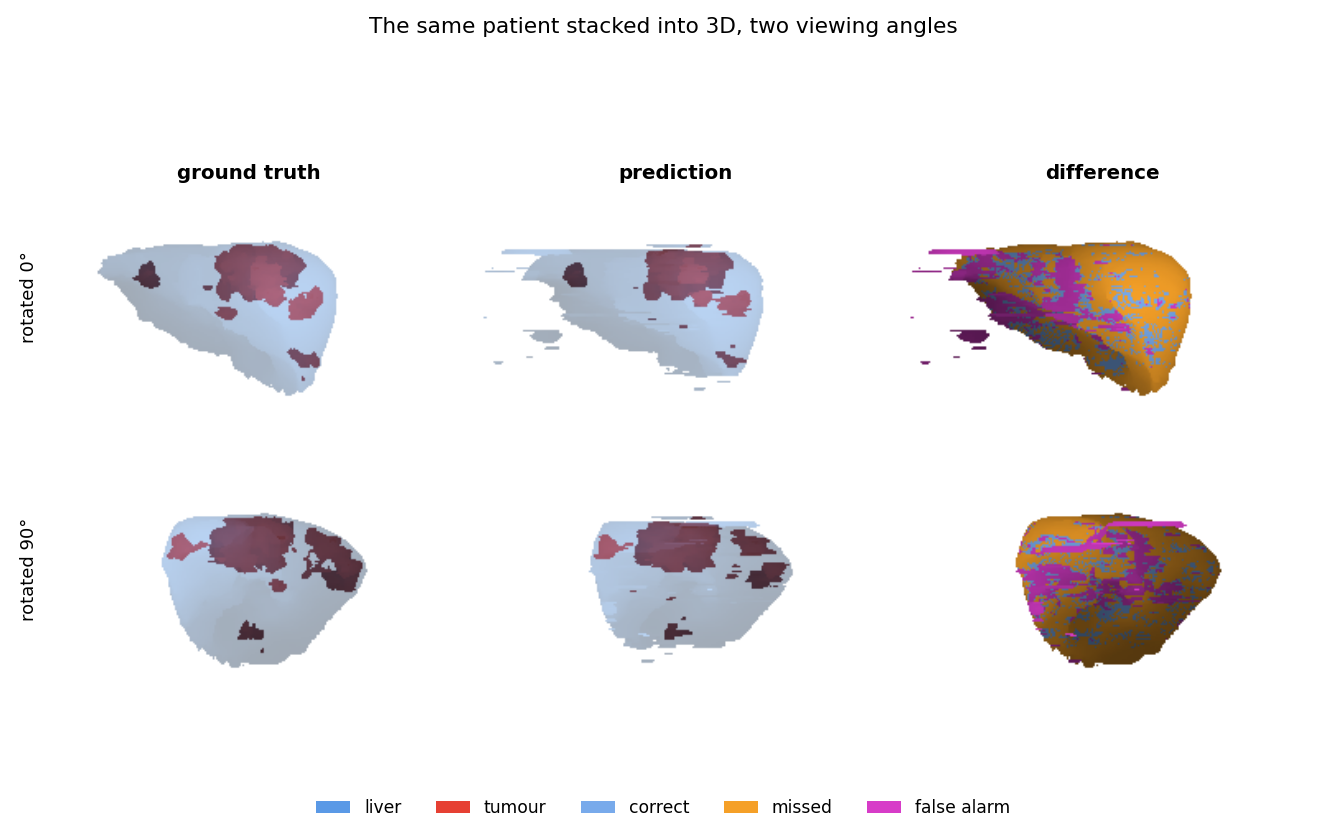
\includegraphics[width=0.92\textwidth]{viewer_volume16_3d.png}
\caption{The same patient in 3D at two angles: ground truth, prediction and the
difference between them.}
\end{figure}

\paragraph{What the 3D view showed.} For patient 16, over the 187 slices with
liver:
\begin{itemize}
  \item correct 812{,}344 voxels, missed 64{,}225, false alarm 30{,}568: the model
        \emph{under}-segments, missing 2.1 times more than it invents;
  \item the missed voxels are not only a thin rim around the outline: 48.9\% of
        them touch a predicted voxel, and 38.7\% are more than two voxels inside
        the true liver, so whole regions were not found;
  \item the prediction is \textbf{23 separate connected pieces}, where the liver
        is one organ. The largest piece (831{,}983 voxels) is 97.5\% inside the
        real liver. The second largest (7{,}634 voxels) does not overlap the liver
        at all; from its position it is most likely the spleen, which has similar
        density on CT.
\end{itemize}

The obvious cleanup is to keep only the largest connected component. I measured
what it would do instead of assuming: it removes 9{,}354 false-positive voxels
(30.6\% of them) but also deletes 1{,}575 correct ones. It is cheap and worth
doing, but most of the error is at the boundary of the organ, not in the stray
pieces. None of this is visible in a per-slice Dice score.

% =====================================================================
\section{Verification tools and engineering problems}\label{sec:eng}
% =====================================================================

\subsection{Checking tools}

Most problems in this work produced no error message, so I wrote small tools whose
only job is to check the rest of the code:

\begin{table}[H]
\centering\small
\begin{tabular}{>{\raggedright}p{3.2cm}p{11cm}}
\toprule
\textbf{Tool} & \textbf{What it checks} \\
\midrule
\code{dataset\_report.py} & slice counts per patient, class balance, mask values, mask nesting, empty slices \\
\code{selftest.py} & nine checks before a long run: clean import path, GPU visible, parameter count matches the diagram, output shape, one $\alpha$ map per gate, patient-level split on real data, batch types and label range, loss and gradients flow, metrics compute \\
\code{summary.py}, \code{diagram.py} & layer tables and diagrams generated from the code, cross-checked so the parameter count agrees in all three places \\
\code{compare.py} & side-by-side table of runs; warns when runs had different epoch budgets \\
\code{attention\_viz.py} & reads out $\alpha$ maps and their selectivity \\
\code{reeval.py} & re-runs the test evaluation on saved checkpoints after a change to the metrics \\
\code{view3d.py}, \code{viewer.py} & 3D reconstruction, NIfTI export, interactive viewer \\
\bottomrule
\end{tabular}
\caption{Verification and analysis tools in the segmentation project.}
\end{table}

\subsection{Problems found, and how}

\begin{table}[H]
\centering\small
\begin{tabular}{>{\raggedright}p{3.6cm}>{\raggedright}p{5.2cm}p{5.4cm}}
\toprule
\textbf{Problem} & \textbf{How it showed up} & \textbf{Fix} \\
\midrule
JPEG-compressed masks & invalid class values in the dataset report & switched to a lossless PNG export \\
slice-level split & scores too good; neighbouring slices in train and test & split by patient \\
accuracy as a metric & 93.4\% for a model that segments nothing & select on foreground Dice \\
unequal training budgets & 0.056 gap between architectures & early stopping off, both 40 epochs \\
interrupted download & results on far fewer test slices & loader refuses mismatched file counts \\
Windows paging-file limit & \code{WinError 1455} with data loader workers & 0 workers on Windows; workers on Linux \\
checkpoint carried Linux settings & same error when re-evaluating on Windows & machine settings overridden on load \\
memory in 3D export & \code{MemoryError} on a 689-slice patient & preallocated 8-bit arrays \\
broken PyTorch install & IDE could not resolve \code{torch.nn} & recreated the conda environment \\
wrong display aspect & liver drawn as a thin sliver & aspect $= z_{\text{scale}}$, not $1/z_{\text{scale}}$ \\
\bottomrule
\end{tabular}
\caption{Silent problems found during the work.}
\end{table}

\paragraph{The Windows memory error.} Each data loader worker is a separate
process that imports PyTorch, and Windows reserves memory for each in the paging
file. With several workers this went over the commit limit and failed with
\code{WinError 1455}. On Linux the same code used several workers without
problems, which is a large part of why the workstation was so much faster.

% =====================================================================
\section{Limitations and future work}\label{sec:lim}
% =====================================================================

\begin{itemize}
  \item \textbf{One run per configuration.} Neither the classification experiments
        nor the architecture comparison are repeated with different seeds, so small
        differences cannot be called significant. Five-fold cross-validation over
        patients would fix this, at the cost of about 20 hours of GPU time.
  \item \textbf{Pooled Dice.} Dice is pooled over all test pixels, so large livers
        count more than small ones. LiTS reports per-patient scores, so my numbers
        are not directly comparable with published results. Per-patient mean and
        standard deviation would be the next metric to add.
  \item \textbf{8-bit 2D export.} The original CT is in Hounsfield units with a much
        wider range than 0--255. The 8-bit PNG export has already lost that, and a
        2D model cannot use context from neighbouring slices.
  \item \textbf{Fixed normalisation.} Mean brightness varies between patients from
        95 to 182, but one fixed normalisation is used for all. Per-image
        normalisation is the first thing I would try.
  \item \textbf{Post-processing.} Keeping the largest connected component removes
        stray pieces such as the probable spleen; I measured its effect on one
        patient but did not apply it to the whole test set.
  \item \textbf{Estimated voxel spacing.} The slice thickness used for 3D display is
        an estimate from the number of slices, not the true value from the scanner.
\end{itemize}

% =====================================================================
\section{Conclusions}
% =====================================================================

On CIFAR-10, a 321-thousand-parameter network reached 88--89\% test accuracy, and
the single-change experiments showed that batch normalisation, depth and
augmentation matter far more than width or dropout. On LiTS, a U-Net and an
Attention U-Net reached the same foreground Dice of about 0.82 under identical
conditions; the attention gates learned to focus on the liver but did not improve
the result. The main weakness of both models is tumour recall of 0.66.

The most useful technical lesson was that almost every serious problem was
silent: damaged labels that still loaded, a split that leaked, a metric that
looked good while the model did nothing, a comparison that measured training time
instead of architecture, and a partial dataset that gave plausible numbers. Each
was found only because a separate check was written for it. Looking at the result
in 3D added information that no single score contained, such as a prediction made
of 23 pieces and a probable spleen labelled as liver.

\appendix

% =====================================================================
\section{Reproducing the results}
% =====================================================================

\paragraph{Classification.}
\begin{verbatim}
conda activate cls
python -m src.train --task binary --epochs 40
python -m src.train --task animals --epochs 50
python -m src.train --task multiclass --epochs 50
python -m src.utils.experiments --task binary --epochs 20   # the ten variants
\end{verbatim}

\paragraph{Segmentation.}
\begin{verbatim}
conda activate seg
python -m src.utils.selftest attention_unet
python -m src.train --arch unet --group ablation_2070
python -m src.train --arch attention_unet --group ablation_2070
python -m src.utils.compare --group ablation_2070
python -m src.utils.view3d --group ablation_2070 --volume 16 --nifti
python -m src.utils.viewer --group ablation_2070 --volume 16
\end{verbatim}

Every run folder contains \code{history.json} with the full configuration and the
per-epoch history, and \code{metrics\_test.json} with the confusion matrix and all
test metrics.

\end{document}
